\hypertarget{ux5f3aux5316ux5faeux8c03}{%
\chapter{强化微调}\label{ux5f3aux5316ux5faeux8c03}}

\hypertarget{ux57faux4e8eux4ebaux7c7bux53cdux9988ux7684ux5f3aux5316ux5b66ux4e60}{%
\section{基于人类反馈的强化学习}\label{ux57faux4e8eux4ebaux7c7bux53cdux9988ux7684ux5f3aux5316ux5b66ux4e60}}

\hypertarget{ux4e00ux4ea7ux751fux80ccux666f}{%
\subsection{一、产生背景}\label{ux4e00ux4ea7ux751fux80ccux666f}}

经过了监督微调以及针对推理的强化微调之后，模型极其聪明，但存在两个问题：

\begin{enumerate}
\def\labelenumi{\arabic{enumi}.}
\item
  难用：可能会中英文夹杂、说话重复、或者语气很冲，因为它只管把题做对，不管人类看着舒不舒服。
\item
  安全性问题：价值观可能未和人类对齐。
\end{enumerate}

\hypertarget{ux4e8cux6838ux5fc3ux539fux7406}{%
\subsection{二、核心原理}\label{ux4e8cux6838ux5fc3ux539fux7406}}

\begin{enumerate}
\def\labelenumi{\arabic{enumi}.}
\tightlist
\item
  奖励模型
\end{enumerate}

我们不可能让人类给所有训练回答打分。因此，我们用一个问题，让模型生成两个（或多个）回答，让人类对这些回答的优劣给出排名，通过回答与排名的对应数据来训练奖励模型。

假设奖励模型参数为 \(\phi\)，对于同一个提示词 \(x\)，有两个回答：

\begin{itemize}
\tightlist
\item
  \(y_w\)（Winner）：人类标注认为更好的回答。
\item
  \(y_l\)（Loser）：人类标注认为较差的回答。
\item
  \(r_\phi(x,y)\)：模型给出的标量分数。
\end{itemize}

损失函数 \(L(\phi)\) 定义为：

\[
L(\phi)=-\mathbb{E}_{(x,y_w,y_l)\sim D}\left[\log\left(\sigma\left(r_\phi(x,y_w)-r_\phi(x,y_l)\right)\right)\right]
\]

其中，\(\sigma\) 是 Sigmoid 函数：

\[
\sigma(z)=\frac{1}{1+e^{-z}}
\]

它将数值压缩到 \((0,1)\) 区间，表示概率。\(r_\phi(x,y_w)-r_\phi(x,y_l)\) 是两者分数的差值。

这实际上是对``模型正确判出更好回答的概率''用了交叉熵损失。上式鼓励了奖励模型给更优的回答给出高分，反之亦然。

这个损失函数本质是对优样本给分大于劣样本的极大似然估计：

根据 Bradley-Terry 模型，这个概率被建模为：

\[
P(y_w>y_l)=\frac{\exp(r(y_w))}{\exp(r(y_w))+\exp(r(y_l))}
\]

将分子分母同时除以 \(\exp(r(y_l))\)，可得：

\[
P(y_w>y_l)=\frac{\exp(r(y_w)-r(y_l))}{1+\exp(r(y_w)-r(y_l))}=\sigma(r(y_w)-r(y_l))
\]

\begin{enumerate}
\def\labelenumi{\arabic{enumi}.}
\setcounter{enumi}{1}
\tightlist
\item
  强化学习
\end{enumerate}

运用强化学习算法如PPO、GRPO，利用第二步的奖励模型为LLM的回答给出奖励，进行强化学习。以PPO为例：

在 RLHF 的 PPO 目标函数中，除了 Clip 这一项，通常还会减去一项 KL 散度（KL 散度实际上是 log 外面加期望，目标函数即 \(R_{\mathrm{total}}\) 整体的期望）：

\[
R_{total}=R_{model}(s,a)-\beta\log\frac{\pi_\theta(a|s)}{\pi_{ref}(a|s)}
\]

第一道锁是 KL Penalty，针对``忘本''与``乱伸''：

\begin{itemize}
\tightlist
\item
  对比对象：当前策略 \(\pi_\theta\) 和 SFT 模型 \(\pi_{ref}\)。
\item
  \(\pi_{ref}\) 是锚：它定格了模型的``老师''或者``出厂设置''（SFT 模型），它在这个训练过程中是永远不变的（Frozen）。
\item
  作用：这是一条长期约束。

  \begin{itemize}
  \tightlist
  \item
    不管训练了多少轮（Epoch），不管你更新了多少次，你都不能偏离``出厂设置''太远。
  \item
    如果不加这一项，模型为了刷分（Reward Hacking），可能会输出乱码或利用 Reward Model 的漏洞。KL 惩罚通过定义``做人话''。
  \end{itemize}
\end{itemize}

第二道锁是 PPO Clip，针对``改革崩坏''：

\begin{itemize}
\tightlist
\item
  对比对象：当前策略 \(\pi_\theta\) 和上一步策略 \(\pi_{\theta_{old}}\)。
\item
  \(\pi_{\theta_{old}}\) 是锚：它是几分钟前的你自己。它是动态变化的。
\item
  作用：这是一条短期约束（步长控制）。

  \begin{itemize}
  \tightlist
  \item
    它保证的是数学上梯度更新的稳定性。它不能保证没有偏离 SFT 模型，它只管``这一次参数更新别太猛''，别把神经网络推崩了。
  \end{itemize}
\end{itemize}

拓展：PPO-Penalty原算法 vs RLHF实际运用时的Penalty

``PPO with Adaptive KL Penalty'' 的变体，它把 KL 直接加在 Loss 函数里。

但在 RLHF 中，我们通常选择把KL``通过每一步的Reward 注入''，而不是直接加在最终的Loss里。这是为了让价值函数V(s)感知到难度，如果把 KL 扣分算在Reward里，那么V(s)在预测``这个状态（生成这个token）好不好''时，就会自动把``偏离SFT模型的代价''也考虑进去。智能体会通过V(s)提前预判到``如果我这就开始乱说话，虽然可能骗到高分，但会被 KL 罚得很惨所以这并不是一个好的状态''。

\hypertarget{ux53c2ux8003ux6587ux732e-77}{%
\subsection{参考文献}\label{ux53c2ux8003ux6587ux732e-77}}

\begin{itemize}
\tightlist
\item
  Ouyang, L., Wu, J., Jiang, X., et al.~(2022). \href{https://arxiv.org/abs/2203.02155}{Training Language Models to Follow Instructions with Human Feedback}. NeurIPS 2022.
\end{itemize}

\clearpage

\hypertarget{dpoux7b97ux6cd5}{%
\section{DPO算法}\label{dpoux7b97ux6cd5}}

DPO算法常用于RLHF。

输入数据是三元组数据集 \(\mathcal{D}=\{x,y_w,y_l\}\)。

模型准备包括：

\begin{itemize}
\tightlist
\item
  \(\pi_\theta\)（Policy Model）：待训练的模型，初始化为 SFT 模型权重。
\item
  \(\pi_{ref}\)（Reference Model）：参考模型，通常就是 SFT 模型的冻结副本，不参与参数更新。
\end{itemize}

在 RLHF 中，我们的目标是最大化期望奖励，同时通过 KL 散度约束模型不要偏离参考模型（SFT 模型）太远。目标函数为：

\[
\max_{\pi}\mathbb{E}_{x\sim D,y\sim\pi(\cdot|x)}[r^*(x,y)]-\beta D_{\mathrm{KL}}(\pi(\cdot|x)\Vert\pi_{ref}(\cdot|x))
\]

其中：

\begin{itemize}
\tightlist
\item
  \(x\)：提示词（Prompt）。
\item
  \(y\)：回复（Response）。
\item
  \(r^*(x,y)\)：真实的、未知的奖励函数。
\item
  \(\pi_{ref}\)：参考模型，通常是 SFT 后的模型。
\end{itemize}

数学上可以证明，上述优化问题的最优解 \(\pi^*\) 具有封闭形式（Closed-form solution）：

\[
\pi^*(y|x)=\frac{1}{Z(x)}\pi_{ref}(y|x)\exp\left(\frac{1}{\beta}r^*(x,y)\right)
\]

其中 \(Z(x)=\sum_y\pi_{ref}(y|x)\exp\left(\frac{1}{\beta}r^*(x,y)\right)\) 是配分函数（Partition Function）。

这是 DPO 最关键的一步。将上式变形并移项，反解出奖励函数 \(r^*(x,y)\)：

\[
r^*(x,y)=\beta\log\frac{\pi^*(y|x)}{\pi_{ref}(y|x)}+\beta\log Z(x)
\]

这个公式表明：如果我们知道了最优策略 \(\pi^*\) 和参考策略 \(\pi_{ref}\)，就可以通过它们比值的对数来表示奖励。

在收集人类偏好数据时，通常是给定一个输入 \(x\) 和两个回复 \((y_w,y_l)\)，其中 \(y_w\) 是胜出（更好）的回复，\(y_l\) 是失败的回复。Bradley-Terry 模型定义了选择 \(y_w\) 的概率：

\[
P(y_w>y_l|x)=\sigma(r^*(x,y_w)-r^*(x,y_l))
\]

其中 \(\sigma\) 是 Sigmoid 函数。

将奖励差写成策略比值形式：

\[
r^*(x,y_w)-r^*(x,y_l)=\beta\log\frac{\pi^*(y_w|x)}{\pi_{ref}(y_w|x)}-\beta\log\frac{\pi^*(y_l|x)}{\pi_{ref}(y_l|x)}
\]

最后，用参数化的模型 \(\pi_\theta\) 来逼近最优策略 \(\pi^*\)。将上述结果代入负对数似然损失（Negative Log Likelihood），得到 DPO 的最终损失函数：

\[
\mathcal{L}_{DPO}(\pi_\theta;\pi_{ref})=-\mathbb{E}_{(x,y_w,y_l)\sim D}\left[\log\sigma\left(\beta\log\frac{\pi_\theta(y_w|x)}{\pi_{ref}(y_w|x)}-\beta\log\frac{\pi_\theta(y_l|x)}{\pi_{ref}(y_l|x)}\right)\right]
\]

直观解释：增加 \(y_w\)（好回复）相较于参考模型的概率比；降低 \(y_l\)（坏回复）相较于参考模型的概率比。\(\beta\) 参数控制了模型偏离参考模型的程度。

也就是说，这两个项的差越大，经过Sigmoid函数后算出的概率也就越大。取负对数，相当于交叉熵损失，让概率预测值尽可能接近1。

\hypertarget{ux53c2ux8003ux6587ux732e-78}{%
\subsection{参考文献}\label{ux53c2ux8003ux6587ux732e-78}}

\begin{itemize}
\tightlist
\item
  Rafailov, R., Sharma, A., Mitchell, E., Manning, C. D., Ermon, S., \& Finn, C. (2023). \href{https://arxiv.org/abs/2305.18290}{Direct Preference Optimization: Your Language Model is Secretly a Reward Model}. NeurIPS 2023.
\item
  Ouyang, L., Wu, J., Jiang, X., et al.~(2022). \href{https://arxiv.org/abs/2203.02155}{Training Language Models to Follow Instructions with Human Feedback}. NeurIPS 2022.
\end{itemize}

\clearpage

\hypertarget{ux4e13ux5bb6ux8fedux4ee3ux4e0eux62d2ux7eddux91c7ux6837}{%
\section{专家迭代与拒绝采样}\label{ux4e13ux5bb6ux8fedux4ee3ux4e0eux62d2ux7eddux91c7ux6837}}

\hypertarget{ux4e00ux4e13ux5bb6ux8fedux4ee3expert-iterationux7684ux57faux672cux601dux60f3}{%
\subsection{一、专家迭代（Expert Iteration）的基本思想}\label{ux4e00ux4e13ux5bb6ux8fedux4ee3expert-iterationux7684ux57faux672cux601dux60f3}}

专家迭代由两个角色组成，它们在一个循环中互相促进：

\begin{enumerate}
\def\labelenumi{\arabic{enumi}.}
\tightlist
\item
  学徒（Apprentice）：即我们要训练的神经网络（Policy \(\pi_\theta\)）。它的特点是推理速度快，但决策质量受限于当前权重。
\item
  专家（Expert）：这通常不是一个外部的人类或更强的模型，而是一个基于当前学徒能力之上的搜索算子（Search Operator）。例如，当前策略加上蒙特卡洛树搜索（MCTS），或者当前策略加上自我采样、重排序、验证器等。专家的特点是计算成本高、速度慢，但通过多步搜索或验证，能产出比学徒质量更高的决策。
\end{enumerate}

算法本质是：学徒通过模仿学习（SFT），学习``如何像专家一样做决策''，从而不需要搜索也能快速得到高质量结果。而在下一轮迭代中，能力变强的学徒又能支撑专家进行更深层的搜索。

阶段 I 是专家生成数据（Expert Improvement）。在这个阶段，我们在固定参数 \(\theta\) 的基础上，利用更消耗计算资源的算法（Expert）来生成优于当前模型直接输出的数据。

假设当前状态为 \(x\)（Prompt），当前模型策略为 \(\pi_\theta\)。我们定义专家算子 \(\Phi\)，它基于 \(\pi_\theta\) 进行增强：

\[
\pi_{expert}(y|x)=\Phi(\pi_\theta,x)
\]

在 LLM 推理场景中，\(\Phi\) 的具体实现通常是：

\begin{itemize}
\tightlist
\item
  搜索（Search）：对同一个 \(x\) 采样 \(N\) 次（Majority Voting），或者进行集束搜索（Beam Search）。
\item
  验证（Verification）：利用单元测试（代码）、或者强化打分器对这些输出正确路径。
\item
  构建数据集（MCTS）：让 AlphaZero 通过构建搜索树来评估每个动作的价值 \(Q(s,a)\) 最高。
\end{itemize}

产出是一批高质量的轨迹数据 \(\mathcal{D}_{new}=\{(x,y_{expert})\}\)，其中 \(y_{expert}\) 是经过搜索验证后的正确推理路径。

阶段 II 是模仿学习（Imitation Learning / Distillation）。在这个阶段，我们将阶段 I 生成的数据 \(\mathcal{D}_{new}\) 视为``标准答案''（Ground Truth），使用监督学习（SFT）来更新模型参数。

目标是最小化 KL 散度，也就是交叉熵损失，让模型的``直觉'' \(\pi_\theta\) 去逼近专家搜索后的分布 \(\pi_{expert}\)：

\[
\theta_{new}=\arg\min_\theta \mathbb{E}_{x\sim D}\left[-\log\pi_\theta(y_{expert}|x)\right]
\]

在 AlphaZero 中，不仅要拟合动作（Policy Head），还要拟合胜率（Value Head）。但在 LLM 推理中，目前主流是只拟合生成的 Token 序列（Policy）。

更新参数的式子看起来是监督学习，实际上却完成了``策略提升''的过程，是给定环境和奖励下的强化学习。当然，前面讲蒙特卡洛树搜索时也讲到过专家迭代思想下不用监督微调的更新方式的方法。

这是一个关键的数学原理：多步搜索通常优于单步预测。

令 \(V(x)\) 为状态 \(x\) 的真实价值（能否解题）。学徒策略 \(\pi_\theta\) 是对最优策略的参数化近似；专家策略 \(\pi_{expert}\) 是基于 \(\pi_\theta\) 进行了 Lookahead（向前看多步）后的改进策略。

根据贝尔曼方程（Bellman Equation）的性质，只要搜索算子 \(\Phi\) 是关于价值函数的``改善算子''（Improvement Operator），那么：

\[
\mathrm{Performance}(\Phi(\pi_\theta))\ge \mathrm{Performance}(\pi_\theta)
\]

Exit 的训练过程就是：

\begin{enumerate}
\def\labelenumi{\arabic{enumi}.}
\tightlist
\item
  \(\pi_{t+1}\approx\Phi(\pi_t)\)（策略更新：让学徒追上专家）。
\item
  \(\pi_{expert}=\Phi(\pi_{t+1})\)（专家基于新学徒再次提升）。
\end{enumerate}

这种螺旋上升的过程，理论上可以让模型最终收敛到该任务的最优解。

\hypertarget{ux4e8cux62d2ux7eddux91c7ux6837ux5faeux8c03rejection-sampling-fine-tuningrft}{%
\subsection{二、拒绝采样微调（Rejection Sampling Fine-Tuning，RFT）}\label{ux4e8cux62d2ux7eddux91c7ux6837ux5faeux8c03rejection-sampling-fine-tuningrft}}

当 SFT 模型具备一定能力后，利用它自己生成数据来进一步提升性能，这被称为专家迭代（Expert Iteration）。

原理：利用 SFT 后的模型对同一个问题 \(x\) 生成 \(k\) 个不同的推理路径 \(\{y_1,y_2,\ldots,y_k\}\)，再利用外部验证器（Rule-based Checker，如 Python 解释器或答案匹配）过滤出结果正确的路径，将这些``模型自己生成的正确路径''加入训练集进行再次微调。

算法工作流：

\begin{enumerate}
\def\labelenumi{\arabic{enumi}.}
\tightlist
\item
  生成（Rollout）：对于数据集中的问题 \(x\)，使用当前策略 \(\pi_\theta\) 采样 \(k\) 个解。设置较高的 temperature 以增加多样性。
\item
  验证（Evaluation）：对于数学题，提取最终答案，与 Ground Truth 比对（Exact Match）；对于代码题，运行 Unit Test。
\item
  过滤与构造：保留通过验证的样本 \((x,y_{correct})\)。
\item
  再训练：将新样本混合入原始 SFT 数据，进行新一轮 SFT。
\item
  迭代：重复上述过程。
\end{enumerate}

\hypertarget{ux4e09starself-taught-reasonerux4eceux9519ux8befux540eux4feeux6b63ux7684ux63a8ux7406ux4e2dux5b66ux4e60}{%
\subsection{三、STaR（Self-Taught Reasoner）：从错误后修正的推理中学习}\label{ux4e09starself-taught-reasonerux4eceux9519ux8befux540eux4feeux6b63ux7684ux63a8ux7406ux4e2dux5b66ux4e60}}

模型生成推理过程和答案。如果答案错误，向模型注入正确答案（Hint），要求模型生成能够推导出正确答案的推理过程（Rationalization）。将这些``后视修正''的推理数据加入训练集，进行监督微调。

\hypertarget{ux56dbux4e13ux5bb6ux8fedux4ee3ux601dux60f3ux7684ux5e94ux7528}{%
\subsection{四、专家迭代思想的应用}\label{ux56dbux4e13ux5bb6ux8fedux4ee3ux601dux60f3ux7684ux5e94ux7528}}

\begin{enumerate}
\def\labelenumi{\arabic{enumi}.}
\tightlist
\item
  LLM
\end{enumerate}

一般如果后续还要用PPO进行针对推理的优化，通常会先跑几轮专家迭代。PPO对初始策略（Initial Policy）很敏感，我们需要一种方式把模型的分布拉到一个较高的水平（SFT后的模型往往还是不够强），再上PPO去优化那些极其困难的Case或进行对齐。专家迭代就适合作为这种方式。而对于GRPO，它是基于组内相对优势更新的，这几个对的样本会产生极大的正向梯度，每一轮更新，模型都在对自己生成的``好样本''进行强化，对``坏样本''进行抑制，实质上起到了专家迭代的作用，免去了``评估搜索结果''这个消耗额外算力的环节。

\begin{enumerate}
\def\labelenumi{\arabic{enumi}.}
\setcounter{enumi}{1}
\tightlist
\item
  AlphaZero
\end{enumerate}

通过原始蒙特卡洛树搜索（而不是针对LLM的改进版本），探索可能的路径。通过交叉熵损失，让策略网络的输出接近蒙特卡洛树搜索方法采样的结果；价值网络拟合的目标价值则直接是最终的输赢结果（只有最终奖励1或-1），即希望输出的预测值v能准确预测最终结果z。

我们希望神经网络输入某个历史状态 \(s_t\) 时，输出的预测值 \(v_t\) 能无限接近最终结果 \(z_t\)。

AlphaZero 的总损失函数包含三部分：价值项、策略项、正则项。其中关于价值更新的部分为均方误差（Mean Squared Error, MSE）：

\[
l_{\mathrm{value}} = (z - v)^2
\]

完整的损失函数为：

\[
\mathcal{L} = \underbrace{(z - v)^2}_{\mathcjk{价值损失}}
- \underbrace{\pi^{T}\log p}_{\mathcjk{策略损失}}
+ \underbrace{c\|\theta\|^2}_{\mathcjk{正则化}}
\]

\begin{itemize}
\tightlist
\item
  \(z\)：这一盘棋最终是谁赢了，是真实结果。
\item
  \(v\)：神经网络在当前状态 \(s\) 预测的赢面。
\end{itemize}

你可能会问：MCTS 搜索得出的 \(Q\) 值不是比网络直接预测的 \(v\) 更准吗？为什么不用 \(Q\) 作为标签来更新 \(v\)？

这是一个很好的直觉，但在 AlphaZero 中：

\begin{itemize}
\tightlist
\item
  Policy Network 的目标是拟合 MCTS 的搜索概率 \(\pi\)，也就是 MCTS 觉得哪一步更好。
\item
  Value Network 的目标是拟合真实结果 \(z\)。
\end{itemize}

原因是：MCTS 的 \(Q\) 值虽然比 \(v\) 准，但它仍然是基于网络预测的 \(v\) 聚合出来的，存在偏差（Bias）。如果让网络去拟合 \(Q\)，相当于``左脚踩右脚''，可能会导致偏差累积。而真实结局 \(z\) 是无偏的（Unbiased），虽然方差大（例如一盘棋赢了不代表这步棋一定好），但只要数据量足够大，网络就能学到最准确的局势判断。

\hypertarget{ux53c2ux8003ux6587ux732e-79}{%
\subsection{参考文献}\label{ux53c2ux8003ux6587ux732e-79}}

\begin{itemize}
\tightlist
\item
  Silver, D., Hubert, T., Schrittwieser, J., et al.~(2018). \href{https://www.science.org/doi/10.1126/science.aar6404}{A general reinforcement learning algorithm that masters chess, shogi, and Go through self-play}. Science.
\item
  Zelikman, E., Wu, Y., Mu, J., \& Goodman, N. (2022). \href{https://arxiv.org/abs/2203.14465}{STaR: Bootstrapping Reasoning With Reasoning}. NeurIPS 2022.
\item
  Silver, D., Huang, A., Maddison, C. J., et al.~(2016). \href{https://www.nature.com/articles/nature16961}{Mastering the game of Go with deep neural networks and tree search}. Nature.
\end{itemize}

\clearpage

\hypertarget{ux57faux4e8eux53efux9a8cux8bc1ux5956ux52b1ux7684ux5f3aux5316ux5b66ux4e60}{%
\section{基于可验证奖励的强化学习}\label{ux57faux4e8eux53efux9a8cux8bc1ux5956ux52b1ux7684ux5f3aux5316ux5b66ux4e60}}

\hypertarget{ux4e00ux6838ux5fc3ux601dux60f3-6}{%
\subsection{一、核心思想}\label{ux4e00ux6838ux5fc3ux601dux60f3-6}}

基于可验证奖励的强化学习（Reinforcement Learning with Varifiable Reward，RLVR）是强化微调的重要范式，使大模型的推理能力实现了飞跃。对于经过预训练的模型，以数学题的答案、编程题的输出结果等的对错或可自动验证的得分作为奖励，可以激发出模型的逻辑推理能力，让模型自行探索出获得正确答案的策略。

这里原则上不引入LLM评分，以免出现Reward Hacking。

\hypertarget{ux4e8cux63d0ux53d6ux7b54ux6848ux7684ux65b9ux5f0f}{%
\subsection{二、提取答案的方式}\label{ux4e8cux63d0ux53d6ux7b54ux6848ux7684ux65b9ux5f0f}}

模型的输出一般为长思维链，包括思考过程（放在\ldots{}标签中）和最终结果（放在\ldots{}标签中）。其中，正确答案默认为最终结果里的最后一个LateX字符串。如果在RL训练初期模型没有遵守格式（例如没有输出标签），系统会直接判定为错误（Reward=0），或者给予一个极小的惩罚。这会迫使模型为了拿到奖励，必须先学会``遵守格式''，然后再学会``做对题目''。

对于数学题，当答案有多种形式时，可用数学公式符号化验证的工具进行判定。对于编程题，可先运行代码，再根据结果给出奖励。对于一些半开放问题如``写出一种满足条件的化学分子式''，答案可能有无数种，可用Checker Script（专用检查脚本）。

\hypertarget{ux4e09ux53efux8bfbux6027ux63d0ux5347}{%
\subsection{三、可读性提升}\label{ux4e09ux53efux8bfbux6027ux63d0ux5347}}

\begin{enumerate}
\def\labelenumi{\arabic{enumi}.}
\tightlist
\item
  硬规则量化：可读性首先需要格式合规性。
\end{enumerate}

（1）结构完整性：是否包含和标签？是否闭合？标签内是否有内容？

（2）重复度：用N-gram 重复率计算，纯RL模型在卡住时很容易陷入死循环（如不断重复``所以\ldots 所以\ldots 所以\ldots{}''）。系统检测生成的文本中n-gram的重复频率，如果超过阈值，给予巨大的负奖励。

（3）语言一致性：用语言检测算法（如fastText）的置信度，如果Prompt是中文，而Chain of Thought中间突然变成了英文或乱码（DeepSeek-R1-Zero 早期经常出现中英夹杂），这被视为可读性差。系统会计算目标语言的token占比，占比越低，惩罚越重。

（4）长度：用Token数量统计，防止模型为了凑字数或者过度推导而生成冗长的废话。通常会有一个软性的长度范围，超出部分会带来微小的负奖励。

\begin{enumerate}
\def\labelenumi{\arabic{enumi}.}
\setcounter{enumi}{1}
\tightlist
\item
  模型量化：奖励模型（Reward Model, RM）
\end{enumerate}

对于逻辑是否通顺、排版是否美观、语气是否像人这种高阶可读性，规则写不出来，于是用另一个模型来打分。这其实就是RLHF（人类反馈强化学习）的思路。

在纯推理模型（如o1或R1）的早期训练阶段，这个比重很低，甚至没有，因为过分追求``好读''可能会损害模型的智商（模型会为了讨好人类而简化复杂的推理步骤）。但在后期这比较重要。

\begin{enumerate}
\def\labelenumi{\arabic{enumi}.}
\setcounter{enumi}{2}
\tightlist
\item
  最关键的手段：SFT``冷启动''与其后的KL散度约束
\end{enumerate}

这可能违背直觉，但实际上，大部分RLVR模型的高可读性，不是在RL阶段练出来的，而是从SFT（监督微调）阶段继承来的。在开始RL之前，模型先通过少量高质量的、人类（或强模型）编写的``完美过程''进行微调。这些数据格式完美、逻辑清晰、语言优雅。而RL训练时，系统会计算当前模型（Policy Model）和SFT模型（Reference Model）之间的KL散度。

如果模型为了解题开始胡言乱语（可读性下降），KL 散度会飙升，导致总奖励下降。这实际上是将可读性隐式地量化为了与人类写作习惯的相似度。

\begin{enumerate}
\def\labelenumi{\arabic{enumi}.}
\setcounter{enumi}{3}
\tightlist
\item
  现实案例：DeepSeek-R1-Zero的教训
\end{enumerate}

DeepSeek 的论文中提供了一个非常精彩的反面教材，证明了如果没有专门的可读性约束，RL 会把可读性彻底毁掉。DeepSeek-R1-Zero没有经过SFT冷启动，没有加可读性奖励，纯RL后模型确实变聪明了，做题正确率飙升，但输出变得极度难以阅读。

\hypertarget{ux53c2ux8003ux6587ux732e-80}{%
\subsection{参考文献}\label{ux53c2ux8003ux6587ux732e-80}}

\begin{itemize}
\tightlist
\item
  DeepSeek-AI. (2025). \href{https://arxiv.org/abs/2501.12948}{DeepSeek-R1: Incentivizing Reasoning Capability in LLMs via Reinforcement Learning}. arXiv:2501.12948.
\item
  《动手学大模型智能体》。
\end{itemize}

\clearpage

\hypertarget{ux5956ux52b1ux51fdux6570ux7684ux6539ux8fdb}{%
\section{奖励函数的改进}\label{ux5956ux52b1ux51fdux6570ux7684ux6539ux8fdb}}

\hypertarget{ux4e00ux9488ux5bf9ux7a00ux758fux5956ux52b1ux95eeux9898ux7684ux4f18ux5316}{%
\subsection{一、针对稀疏奖励问题的优化}\label{ux4e00ux9488ux5bf9ux7a00ux758fux5956ux52b1ux95eeux9898ux7684ux4f18ux5316}}

RLVR依赖可验证的奖励信号（如数学题的答案、编程题的输出结果）来指导，这是非常稀疏的。只有当智能体生成的代码从头到尾（数据加载、训练、预测、生成提交文件）完美运行时，才能得到一个非零的分数。一个因为数据加载失败的程序和一个几乎成功、仅在最后保存文件时出错的程序，得到的奖励都是零（或者是一个表示失败的固定负值）。这使得智能体难以获得有效梯度（特别是难题），即很难区分``错得离谱''和``就差一点''这两种情况，导致学习效率低下。可能的优化方案：

\begin{enumerate}
\def\labelenumi{\arabic{enumi}.}
\tightlist
\item
  融合步骤分解与密集反馈
\end{enumerate}

核心思想是给AI的每一步操作都打上``进度条''，让其输出中间变量，从而可以更密集地给予奖励，使得AI不至于在前期完全没有梯度。

但注意：一般后期正确率达到一定水平后会切换回纯结果奖励，确保AI不会止步于局部最优，而是探索完全正确的答案。

（1）中间步骤输出（硬性打分）

自动注入代码：在智能体生成的代码执行前，利用一个独立的静态语言模型，自动向代码中插入一系列中间输出语句，例如：print(``loaded data''), print(``trained model'')。

解析输出以计分：代码执行后，系统通过正则表达式（Regex）扫描终端输出日志，检测哪些中间变量被成功打印。

分级奖励结构：每输出一个正确中间变量，智能体获得一小部分奖励（如+0.1分）。

优势：即使程序最终失败，智能体也能获得有指导性的反馈，被逐步引导先学会加载数据，再学会构建模型，最终完成任务。而且这里的奖励一般情况下较为可验证、客观。

（2）过程思路评分（LLM打分）

不要只依赖结果，也需要关注过程思路，如果思维链（CoT）合理但计算错误，仍可给予部分分数。这种方法就像高考数学大题阅卷一样，即便答案错，只要思路对，仍然可以得到大部分分数，也就是按思路过程评分；只有结果没有过程，不能得到大部分分数。

在过程的评分中，可以引入结构性检查，如数学任务检查是否包含关键的中间变量、还原步骤，程序任务检测是否使用了题目规定的函数名、变量名等。

但注意，这种思路可能要谨慎使用。因为它不是有明确标准的RLVR。LLM的泛化能力不是无限的，在评价标准比较主观灵活的情况下（如按过程思路而非单纯按答案给分），在RL的范式智能体很可能找到一个``Reward Hacking''的方式，而且这种对抗性样本的漏洞不可能全部被完美堵上。

\begin{enumerate}
\def\labelenumi{\arabic{enumi}.}
\setcounter{enumi}{1}
\tightlist
\item
  为什么要慎用（如只能在前期使用）过程奖励
\end{enumerate}

前面的方法虽然能解决训练难的问题，但解决真实问题时或在真实环境中，奖励信号稀疏本就是内在特征（如生物进化以存活数量为奖励），我们人为把奖励改得更密集，从原理上无法根避开优化目标发生了变化这一根本问题。如果AI用了一种人类根本不懂的绝妙方法（比如AlphaGo的第37手），反而可能被错误地打低分。

另外，奖励过于密集，也容易让模型过度看重即时奖励，陷入局部最优，降低在依赖长期规划和一致性的任务上的效果，就如同对科研人员的考核如果过于频繁，会引导人们一味做短平快研究，降低出重大成果的可能性一样。具有一定程度稀疏性的奖励本来就是更为本质的。

综上，一般而言如果希望通过过程奖励解决奖励稀疏问题，一般只在前期运用过程奖励。当奖励达到阈值后，切换为纯结果奖励。

\begin{enumerate}
\def\labelenumi{\arabic{enumi}.}
\setcounter{enumi}{1}
\tightlist
\item
  SRL（监督式强化学习）（Google，2025）
\end{enumerate}

对于不够聪明的模型，让它死记硬背高质量答案（SFT）反而会把它教傻；相反，可以像一位耐心导师一样，把难题拆解成小步骤，模型每做一步就对照标准答案给``相似分''，通过这种``手把手+鼓励式''教学，成功让小模型学会了它本不可能掌握的复杂推理。

SRL不再把一个完整的解题过程看作一个整体，而是将其分解为一系列关键的``动作''（Action）。在生成每个``动作''之前，模型会先生成一段``内心独白''，放在标签里。这个设计非常巧妙，它把灵活的思考过程和需要被评估的、结构化的执行步骤分开了。

在模型完成每一步``动作''后，系统会将其与专家示范中的对应``动作''进行文本相似度比较，得出一个0到1之间的分数作为奖励。这意味着即使模型的一步做得不完美，只要方向大致正确，也能得到正向的反馈。这种``差不多就行，有点像就好''的奖励机制，为模型在复杂的探索空间中提供了一个平滑的、连续的学习信号。

为了提高训练效率，SRL会过滤掉那些几乎所有尝试的相似度分数都差不多、学习信号很弱的训练样本。

该方法一般在强化微调前期应用，或者在借助大模型训练小模型时应用。大模型强化学习后期仍采取RLVR，以激发更大的潜能，让它探索和发现新方法。

\begin{enumerate}
\def\labelenumi{\arabic{enumi}.}
\setcounter{enumi}{2}
\tightlist
\item
  目标导向的强化学习
\end{enumerate}

具体介绍见目标导向的强化学习一节。这里举一些在强化微调中应用的例子。

数学题求解中：

\begin{itemize}
\tightlist
\item
  原始目标 \(g\)：计算 \(\int x^2 dx\)。
\item
  模型行为：模型错误地计算成了 \(\frac{1}{2}x^2\)，可能忘记了系数 \(\frac{1}{3}\)，或者是对 \(x\) 求导了。
\item
  传统方法：判断错误，奖励为 0。
\item
  Goal-Oriented 方法：

  \begin{itemize}
  \tightlist
  \item
    分析模型输出 \(\frac{1}{2}x^2\)。
  \item
    逆向推导或重标记：这其实是问题``计算 \(\int x dx\)''的正确答案，或者是``计算 \(\frac{1}{6}x^3\) 的导数''的答案。
  \item
    更新：告诉模型，``如果你想解决计算 \(\int x dx\) 这个问题，你的刚才的推导是完美的。''
  \item
    效果：模型学会了正确的积分逻辑，只是最初用错了地方。
    代码生成中：
  \end{itemize}
\item
  原始目标 \(g\)：加载数据并训练模型。
\item
  模型行为：成功加载了数据，但在训练模型时报错崩溃。
\item
  重标记 \(g'\)：将目标修改为``编写一个数据加载脚本''。
\item
  结果：在这条新轨迹下，模型获得了满分。它强化了``如何正确加载数据''的能力。
\end{itemize}

\begin{enumerate}
\def\labelenumi{\arabic{enumi}.}
\setcounter{enumi}{3}
\tightlist
\item
  从中间状态开始推理
\end{enumerate}

在RLVR训练中，模型经常会产生一些部分正确的推理链。HiPO提取这些成功或部分成功轨迹的前缀作为``提示（Hint）''，强制模型从这些有希望的中间状态继续探索。这实际上是将一个长程的稀疏奖励问题分解成了若干个短程的条件生成问题，人为地增加了获得奖励的频率。

\begin{enumerate}
\def\labelenumi{\arabic{enumi}.}
\setcounter{enumi}{4}
\tightlist
\item
  改进RL算法
\end{enumerate}

RL算法的改进也能让稀疏的奖励信号更好地回传，如GRPO在这点上优于PPO（后者的Critic网络可能在稀疏奖励下训练极不稳定）。这样也能让模型更好地适配真实世界中往往本就奖励稀疏的实际情况。

\hypertarget{ux4e8cux7b54ux6848ux683cux5f0fux7684ux8c03ux6574}{%
\subsection{二、答案格式的调整}\label{ux4e8cux7b54ux6848ux683cux5f0fux7684ux8c03ux6574}}

\begin{enumerate}
\def\labelenumi{\arabic{enumi}.}
\tightlist
\item
  HERO：将结果奖励与格式奖励结合（Meta FAIR，2025）
\end{enumerate}

先定性，由0-1二值分类的验证器，将所有答案分为``正确''和``错误''两组（定性阶段），通过分层归一化将所有模型输出按对错分组，确保奖励分数不越界。然后再定量，让奖励模型在每个组的内部，对答案的质量进行精细的排序，给出质量的细微分数，通过方差感知加权，让模型在训练时更关注那些信息量最大的难题。这样，``格式差的正确答案''的得分高于一个``格式好的错误答案''，优先保证训练的方向正确。

\hypertarget{ux4e09ux8f93ux51faux7ed3ux679cux7684ux7b49ux4ef7ux6027ux5206ux6790}{%
\subsection{三、输出结果的等价性分析}\label{ux4e09ux8f93ux51faux7ed3ux679cux7684ux7b49ux4ef7ux6027ux5206ux6790}}

针对数学推导任务（特别是化简表达、解题过程不唯一的场景），我们不能单纯比较输出字符串与答案是否匹配，需要更贴近数学本质的奖励定义方式。如Symbolic Equivalence（符号等价）调用符号计算工具（如Python的SymPy库）判断两个表达式在数学上是否等价。相较于直接比较模型输出与标准答案是否完全一致，符号等价具有更强的泛化性，更能反映数学推理的正确性。

\hypertarget{ux56dbux89e3ux51b3ux6a21ux578bux4f5cux5f0aux8499ux7b54ux6848ux95eeux9898}{%
\subsection{四、解决模型``作弊''蒙答案问题}\label{ux56dbux89e3ux51b3ux6a21ux578bux4f5cux5f0aux8499ux7b54ux6848ux95eeux9898}}

适当加入对过程的检查。在代码执行环境中，禁止import某些危险函数（如eval），禁止直接打印答案等。

\hypertarget{ux4e94ux5197ux4f59ux8f93ux51faux95eeux9898}{%
\subsection{五、冗余输出问题}\label{ux4e94ux5197ux4f59ux8f93ux51faux95eeux9898}}

在推理中，模型常会出现``过度思考''问题，为了得出一个简单的结论，生成大量冗余Token，甚至在多种错误的路径上反复横跳，或者不断回溯。这不仅浪费了宝贵的算力，还增加了推理延迟。

可能的解决方案：

\begin{enumerate}
\def\labelenumi{\arabic{enumi}.}
\tightlist
\item
  直接修改RL算法的目标函数
\end{enumerate}

有时模型输出冗余token，可能是因为奖励函数的设计还需要优化。如DeepSeek-V3.2生成大量冗余token的问题就和GRPO的目标函数里把奖励期望除以T，变成了每个token奖励的期望直接相关。通过修改目标函数的形式，能一定程度上缓解该问题。

\begin{enumerate}
\def\labelenumi{\arabic{enumi}.}
\setcounter{enumi}{1}
\tightlist
\item
  RePro（上海AI Lab，2025）
\end{enumerate}

（1）核心观察：推理即优化

RePro的核心思想是将模型的推理轨迹看作是在损失曲面上寻找最优解的路径。

每一个推理步骤（Step），都相当于一次梯度更新。优化的目标，是最大化生成正确答案（Ground Truth）的概率。好的推理，应该每一步都能显著提升模型对正确答案的信心（Loss下降），且推理方向坚定，不反复横跳，不震荡。过度思考，则体现为陷入鞍点（生成了大量Token，但对正确答案概率提升的贡献微乎其微），或梯度震荡（思路混乱，信心忽高忽低）。

基于上述视角，RePro设计了一套过程奖励机制，直接嵌入到RLVR（如PPO，GRPO）流程中。

（2）代理目标函数

RePro设计了一个目标函数，用于量化模型当前的置信度。具体来说，即模型在当前推理上下文下，生成正确答案各个token的平均对数概率。（和监督学习中的分类损失有相似之处）

\[
\tilde{J}(\pi_\theta, q, \tau_{\le t}, a)
\triangleq
\frac{1}{|a|}\sum_{i=1}^{|a|}
\log \pi_\theta(a_{(i)} \mid q, \tau_{\le t})
\]

当模型还没开始思考时，直接猜出答案的概率很低，J̃很小。随着模型一步步推理，排除错误选项，锁定逻辑链路，模型对最终答案的信心应该越来越强，J̃应该逐渐增大。当模型完成推理得出结论时，J̃应该达到峰值。这个指标越高，说明模型越``自信''答案正确，是一个合理的优化指标。

（3）基于J序列引入的两个评分

相较于传统强化学习仅关注最终结果（Outcome Reward）的稀疏反馈机制，REPRO引入了过程感知的轨迹优化范式。为了量化推理质量，RePro将J̃的变化拆解为两个维度：

Magnitude Score（强度评分）衡量目标函数变化幅度，旨在回答``这一段思考，到底让模型离答案近了多少''。在优化理论中，梯度的大小决定了下降的快慢。在推理中，这意味着一段有效的CoT应该显著提升模型对答案的信心。REPRO通过比较当前步骤后的目标函数值J̃与基线值J̅（即不进行任何思考直接回答的信心）来计算这一增益。

\[
\Delta(\pi_\theta, q, \tau_{\le t}, a)
=
\frac{
\tilde{J}(\pi_\theta, q, \tau_{\le t}, a) - \bar{J}_b(q)
}{
\bar{J}_b(q)
}
\]

\[
S_{\mathrm{magn},(t)}
\triangleq
\tanh\left(\Delta(\pi_\theta, q, \tau_{\le t}, a) + 1\right) + 1
\]

这里使用tanh函数的目的是将分数归一化到(0,1{]}区间。在实际训练中，某些步骤可能会导致对答案的信心指数级暴涨（例如终于算出了关键中间变量），如果不加限制，这种巨大的奖励信号可能会导致梯度爆炸或训练不稳定。

Stability Score（稳定性评分）衡量J是否平滑上升。如果将J̃的变化看作一条曲线，理想的推理应该是一条单调上升的曲线。如果曲线上下波动，说明模型陷入了自我怀疑或逻辑混乱。为了量化这种``波动''，RePro利用了Kendall's Tau相关系数。

\[
S_{\mathrm{stab},(t)}
=
\frac{
\sum_{i < j}
\mathrm{sign}(\tilde{J}_i - \tilde{J}_j)\cdot \mathrm{sign}(i - j)
}{
|\tau|(|\tau| - 1)
}
+
\frac{1}{2}
\]

这一公式计算的是J̃值序列与时间步序列\{1,\ldots,t\}之间的秩相关性。高稳定性（接近1）意味着每一步的J̃值都比前一步高，这表明模型每一步都在进步，没有回撤。这对应于优化过程中沿着最速下降方向的平滑移动。低稳定性（接近0或负值）意味着序列杂乱无章，进两步退一步，甚至出现严重的逻辑倒退。这对应于模型在鞍点附近的随机摆动，消耗了步数（Token）但未取得实质进展。

Magnitude Score和Stability Score两者加权构成最终过程评分S，可用于判断某段思维路径是否值得强化或惩罚。

（4）流程级奖励

RePro采用熵值筛选策略：

分段：将推理链按逻辑段落（如换行符\n\n）分割为\{c1, c2,\ldots, cN\}。

熵计算：计算每个段落首 Token 的熵 \(\mathcal{H}(c_i^{(0)})\)。

Top-k 筛选：只选择熵最高的前 \(k\) 个段落（Top-k Segments）进行 REPRO 奖励计算。

这种策略不仅大幅降低了计算开销（从全序列计算变为只计算 \(k\) 个点），还起到了``好钢用在刀刃上''的效果------只在模型最迷茫、最关键的时刻给予指引，而在其自信流畅的时刻（低熵区域）保持静默，避免过度干预。

然后，通过计算过程评分的提升量 \(\Delta S\)，作为这一片段的``过程级奖励''，与最终正确与否结合，作为 RL 的优势函数输入。

\hypertarget{ux53c2ux8003ux6587ux732e-81}{%
\subsection{参考文献}\label{ux53c2ux8003ux6587ux732e-81}}

\begin{itemize}
\tightlist
\item
  《动手学大模型智能体》。
\item
  Deng, Y., Hsu, I.-H., Yan, J., et al.~(2025). \href{https://arxiv.org/abs/2510.25992}{Supervised Reinforcement Learning: From Expert Trajectories to Step-wise Reasoning}. arXiv:2510.25992.
\item
  Tao, L., Kulikov, I., Saha, S., et al.~(2025). \href{https://arxiv.org/abs/2510.07242}{Hybrid Reinforcement: When Reward Is Sparse, It's Better to Be Dense}. arXiv:2510.07242.
\item
  Liu, J., Liu, H., Zhang, S., \& Chen, K. (2025). \href{https://arxiv.org/abs/2512.01925}{Rectifying LLM Thought from Lens of Optimization}. arXiv:2512.01925.
\end{itemize}

\clearpage

\hypertarget{ppoux7b97ux6cd5ux5728ux5f3aux5316ux5faeux8c03ux4e2dux7684ux5e94ux7528}{%
\section{PPO算法在强化微调中的应用}\label{ppoux7b97ux6cd5ux5728ux5f3aux5316ux5faeux8c03ux4e2dux7684ux5e94ux7528}}

\hypertarget{ux4e00ppoux7b97ux6cd5ux7684ux76eeux6807ux51fdux6570ux548cux524dux9762ux5728ux5f3aux5316ux5b66ux4e60ux90e8ux5206ux4e2dux4ecbux7ecdux7684ux76f8ux540c}{%
\subsection{一、PPO算法的目标函数（和前面在强化学习部分中介绍的相同）}\label{ux4e00ppoux7b97ux6cd5ux7684ux76eeux6807ux51fdux6570ux548cux524dux9762ux5728ux5f3aux5316ux5b66ux4e60ux90e8ux5206ux4e2dux4ecbux7ecdux7684ux76f8ux540c}}

策略的目标函数：

\[
r_t(\theta)=\frac{\pi_\theta(a_t \mid s_t)}{\pi_{\theta_{\mathrm{old}}}(a_t \mid s_t)}
\]

\[
J^{\mathrm{CLIP}}(\theta)
=
\mathbb{E}_t\left[
\min\left(
r_t(\theta)A_t,
\mathrm{clip}(r_t(\theta), 1-\epsilon, 1+\epsilon)A_t
\right)
\right]
\]

其中：

\begin{itemize}
\tightlist
\item
  \(r_t(\theta)\)：新策略与旧策略在动作 \(a_t\) 上的概率比。
\item
  \(A_t\)：当前动作的优势估计，表示它相对平均水平好多少。
\item
  \(\epsilon\)：裁剪范围，用来限制策略更新幅度。
  价值 \(A_t\) 的估计方法：
\end{itemize}

如果我们只看一步未来，那么动作 \(a_t\) 的 \(Q\) 值可以被估计为 \(r_t + \gamma V(s_{t+1})\)。此时，\(A_t\) 的估计值直接等于 TD Error：

\[
\hat{A}_t^{(1)}
=
\underbrace{r_t + \gamma V(s_{t+1})}_{\approx Q(s_t,a_t)}
- V(s_t)
=
\delta_t
\]

PPO 默认使用 GAE 来计算优势函数。这个设计非常精妙，它将 TD Error 进行了指数加权移动平均：

\[
\hat{A}_t^{\mathrm{GAE}}
=
\delta_t
+
(\gamma\lambda)\delta_{t+1}
+
(\gamma\lambda)^2\delta_{t+2}
+
\cdots
\]

其中 \(\lambda\) 是范围在 \([0,1]\) 之间的超参数。

通过 \(\lambda\) 调节 TD Error 的作用：

\begin{itemize}
\tightlist
\item
  当 \(\lambda = 0\) 时，高偏差、低方差：
\end{itemize}

\[
\hat{A}_t = \delta_t = r_t + \gamma V(s_{t+1}) - V(s_t)
\]

此时 \(A_t\) 完全等于当前的单步 TD Error。

\begin{itemize}
\tightlist
\item
  优点：方差小，只依赖一步随机奖励 \(r_t\)。
\item
  缺点：偏差大，严重依赖 Critic 网络 \(V(s_{t+1})\) 的准确性；如果 Critic 没训练好，估计就是错的。
\item
  当 \(\lambda = 1\) 时，无偏差、高方差：
\end{itemize}

\[
\hat{A}_t
=
\sum_{l=0}^{\infty}\gamma^l\delta_{t+l}
=
\left(\sum_{l=0}^{\infty}\gamma^l r_{t+l}\right)
- V(s_t)
\]

此时公式展开后，中间的 \(V\) 项会相互抵消，最终变成 Monte Carlo Returns（真实回报）减去 Baseline。

\begin{itemize}
\tightlist
\item
  优点：偏差小，真实回报是最准确的``事实''。
\item
  缺点：方差极大，因为累加了每一步环境的随机性。
  \#\#\# 二、PPO算法运用于强化微调的工作流（和前面介绍的略有不同）
\end{itemize}

\begin{enumerate}
\def\labelenumi{\arabic{enumi}.}
\tightlist
\item
  数据采集阶段
\end{enumerate}

在机器人控制等传统RL的环境中，智能体连续与环境持续交互（如2048次），形成一条长轨迹序列，后续再将序列随机打乱成小批量计算梯度。但LLM微调中的PPO使用的是向量化环境，我们可以并行处理一系列Prompt，各自并行生成轨迹并存入Replay Buffer：

``2048 步''实际上是所有并行环境生成的 Token 总数。

假设你的显卡并行能力允许你同时处理 \(N\) 个 Prompt（并行环境数，比如 \(N = 16\)）。

\begin{itemize}
\tightlist
\item
  时刻 \(t = 1\)：模型同时看到了 16 个不同的 Prompt，并发出了 16 个 Token（每个 Prompt 一个）。这在计数器上算作 16 个 Steps。
\item
  时刻 \(t = 2\)：模型基于之前的 Token，又并发生成了 16 个 Token。
\item
  以此类推。
\end{itemize}

计算公式是：

\[
\text{Total Steps }(2048)
=
\mathcjk{并行 Prompt \mathcjk{数量}}
\times
\mathcjk{每个回复的平均长度}
\]

举个例子：如果图片里写``运行 2048 步''，它实际上可能发生了以下情况：

\begin{enumerate}
\def\labelenumi{\arabic{enumi}.}
\tightlist
\item
  系统从数据集里抽出了 16 个不同的 Prompt。
\item
  模型对这 16 个 Prompt 并行生成回答。
\item
  每个回答平均生成了 128 个 Token 就结束了。
\item
  总收集的数据量（Steps）为 \(16 \times 128 = 2048\)。
\end{enumerate}

所以，这 2048 步里包含了 16 个不同 Prompt 的完整故事，而不是 1 个 Prompt 的超长故事。
2. 优势计算阶段（和传统RL中一致）

初始化：初始化 Actor 网络 \(\pi_\theta\) 和 Critic 网络 \(V_\phi\)。

大循环（For each iteration）：

\begin{enumerate}
\def\labelenumi{\arabic{enumi}.}
\tightlist
\item
  数据收集阶段（Interaction）：

  \begin{itemize}
  \tightlist
  \item
    使用当前策略 \(\pi_{\theta_{\mathrm{old}}}\) 在环境中运行 \(T\) 步，例如 2048 步。
  \item
    收集轨迹数据：\(\{s_t, a_t, r_t, s_{t+1}, \log \pi_{\theta_{\mathrm{old}}}(a_t \mid s_t)\}\)。
  \item
    利用 Critic 网络计算状态价值 \(V(s_t)\)。
  \end{itemize}
\item
  优势计算阶段（Advantage）：

  \begin{itemize}
  \tightlist
  \item
    计算 TD Error：\(\delta_t = r_t + \gamma V(s_{t+1}) - V(s_t)\)。
  \item
    计算 GAE（Generalized Advantage Estimation）\(A_t\)。这是一个递归公式，用来在偏差和方差之间做平衡。
  \end{itemize}
\item
  优化更新、同步策略阶段
\end{enumerate}

收集阶段：显卡像收割机一样，通过并行处理很多 Prompt，迅速填满一个容量为 2048 的经验池（Replay Buffer）。这个池子里面能混杂了 16 个不同问题的问答记录。

打乱（Shuffle）：为了训练稳定、打破数据之间的相关性，我们把这 2048 个 Token（数据点）彻底打乱。

切分（Mini-batch）：把打乱后的 2048 个数据切分成小块，例如 Batch Size 为 64。

\begin{itemize}
\tightlist
\item
  这意味着 \(2048 / 64 = 32\) 个 Mini-batches。
\item
  模型会用这 32 个小批次来更新参数。
\end{itemize}

\begin{enumerate}
\def\labelenumi{\arabic{enumi}.}
\setcounter{enumi}{2}
\tightlist
\item
  优化更新阶段（Optimization）：
\end{enumerate}

\begin{itemize}
\tightlist
\item
  重要：此时 \(\pi_{\theta_{\mathrm{old}}}\) 固定不动，作为分母；我们优化的是新的 \(\pi_\theta\)，作为分子。
\item
  将收集到的 \(T\) 个数据打乱，分成多个 Mini-batch，例如每个 batch 64 个数据。
\item
  Epoch 循环，例如重复 10 次：

  \begin{enumerate}
  \def\labelenumi{\arabic{enumi}.}
  \tightlist
  \item
    对每个 Mini-batch，计算新概率比率 \(r_t(\theta)=\frac{\pi_\theta(a \mid s)}{\pi_{\theta_{\mathrm{old}}}(a \mid s)}\)。
  \item
    计算 Clip 损失 \(L^{\mathrm{CLIP}}\)。
  \item
    计算 Critic 的价值损失 \(L^{\mathrm{VF}} = (V_\phi(s_t) - V_{\mathrm{target}})^2\)。
  \item
    计算熵正则项 \(S\)，鼓励探索。
  \item
    总损失：\(L = -L^{\mathrm{CLIP}} + c_1 L^{\mathrm{VF}} - c_2 S\)。注意梯度上升/下降符号。
  \item
    反向传播更新 \(\theta\) 和 \(\phi\)。
  \end{enumerate}
\end{itemize}

\begin{enumerate}
\def\labelenumi{\arabic{enumi}.}
\setcounter{enumi}{3}
\tightlist
\item
  同步策略：
\end{enumerate}

\begin{itemize}
\tightlist
\item
  本轮更新结束，令 \(\pi_{\theta_{\mathrm{old}}} \leftarrow \pi_\theta\)。
\item
  清空数据缓冲区，进入下一次大循环。
\end{itemize}

\hypertarget{ux4e09llmux4e3aux4f55ux9009ux62e9ppoux800cux975esacux4e3aux4f55ux9009ux62e9on-policyux800cux975eoff-policy}{%
\subsection{三、LLM为何选择PPO而非SAC？为何选择On-Policy而非Off-Policy？}\label{ux4e09llmux4e3aux4f55ux9009ux62e9ppoux800cux975esacux4e3aux4f55ux9009ux62e9on-policyux800cux975eoff-policy}}

\hypertarget{ux4e00llmux8f93ux51faux79bbux6563ux800cux975eux8fdeux7eedux52a8ux4f5c}{%
\subsubsection{（一）LLM输出离散而非连续动作}\label{ux4e00llmux8f93ux51faux79bbux6563ux800cux975eux8fdeux7eedux52a8ux4f5c}}

SAC 的原生设计：SAC 是为连续动作空间（Continuous Action Space）设计的最大熵强化学习算法。在机器人控制中，动作是关节的角度或力矩（实数值）。虽然存在 Discrete SAC 的变体，但在处理高维离散空间时，计算成本极高。

LLM 的场景：LLM 的生成过程是在一个巨大的词表（Vocabulary）中选择下一个 Token。

\begin{itemize}
\tightlist
\item
  动作空间大小 \(|A|\)：通常在 \(32,000\) 到 \(128,000\) 甚至更大，例如 GPT-4 或 Qwen 的词表。
\item
  维度灾难：在 Actor-Critic 架构中，Critic 网络需要评估动作价值 \(Q(s,a)\)。

  \begin{itemize}
  \tightlist
  \item
    对于 Discrete SAC，为了计算目标值（Target \(Q\)）和策略的熵，通常需要对所有可能的动作进行边缘化（Marginalization）或 Softmax 计算。
  \item
    公式会涉及计算 \(\pi(a' \mid s') \cdot [Q(s',a') - \alpha \log \pi(a' \mid s')]\) 的期望，也就是：
  \end{itemize}
\end{itemize}

\[
\mathbb{E}_{a'\sim \pi(\cdot \mid s')}
\left[
Q(s',a')-\alpha\log\pi(a'\mid s')
\right]
=
\sum_{a'\in A}\pi(a'\mid s')
\left[
Q(s',a')-\alpha\log\pi(a'\mid s')
\right]
\]

这意味着每一步更新都要对 \(50,000+\) 个 Token 做全概率计算，在计算上极其昂贵。

那或许你会说，既然词表大小高达 10 万，那么它看起来确实很像一个连续空间。如果我们把Policy的输出改成一个连续嵌入向量，而不是一个10万维的概率分布，显存和计算量岂不是大大降低？但在实践中，这条路目前被证明是走不通的。

\begin{enumerate}
\def\labelenumi{\arabic{enumi}.}
\tightlist
\item
  ``梯度阻断''：如何在离散的悬崖上求导？
\end{enumerate}

这是最核心的数学死结。

\begin{itemize}
\tightlist
\item
  连续动作的假象：假设 Actor 网络输出一个连续向量 \(\mathbf{v}\in\mathbb{R}^d\)，例如 \(d=4096\)。为了把这个向量输入给环境，或者用来预测下一个 Token，必须把它映射回真实词表。
\item
  最近邻搜索（Nearest Neighbor Search）：必须在 Embedding Table 中找到与 \(\mathbf{v}\) 距离最近的那个 Token Embedding \(\mathbf{e}_k\)：
\end{itemize}

\[
k
=
\underset{j\in V}{\arg\min}\,
\lVert \mathbf{v}-\mathbf{e}_j\rVert_2
\]

\begin{itemize}
\tightlist
\item
  梯度的噩梦：这个 \(\arg\min\) 操作不可导，或者说梯度几乎处处为 0。

  \begin{itemize}
  \tightlist
  \item
    如果输出向量 \(\mathbf{v}\) 在空间中只移动一点点，且没有跨过最近邻边界，最近邻 Token 仍然是 \(k\)，此时梯度为 0，因为输出不变，Loss 不变。
  \item
    如果它突然跨过边界，最近邻变成了 Token \(m\)，这又是阶跃跳变（Step Function），导数无穷大或未定义。
  \end{itemize}
\end{itemize}

没有梯度，反向传播就断了，Actor 网络学不到任何东西。虽然有 Gumbel-Softmax 这样的松弛技巧（Relaxation），但在 10 万维空间中，它的方差极大，训练极其不稳定。

\begin{enumerate}
\def\labelenumi{\arabic{enumi}.}
\setcounter{enumi}{1}
\tightlist
\item
  ``无人区''问题：Embedding 空间的稀疏性
\end{enumerate}

你可能会想：``那我不要 argmax，我直接把输出的连续向量 \(\mathbf{v}\) 喂给下一层网络不就行了？''

这里涉及流形假设（Manifold Hypothesis）。

\begin{itemize}
\tightlist
\item
  词向量不是均匀分布的：在 4096 维的高维空间中，有效的 Token Embedding 只占据极小的一部分点（Point Cloud）。绝大多数空间都是无效的空白区域（Void Space），也就是所谓的``无人区''。
\item
  连续控制的灾难：RL 的探索（Exploration）通常是在动作上加高斯噪声。如果在连续向量 \(\mathbf{v}\) 上加噪声，你会大概率落入``无人区''。

  \begin{itemize}
  \tightlist
  \item
    结果：这个向量既不像``苹果''，也不像``香蕉''，而是一个没有任何语义信息的杂乱向量。
  \item
    语言模型崩塌：当你把这个无意义的向量传给下一层，整个 Transformer 的注意力机制就会处理混乱的信息，导致后续生成的全是乱码。
  \end{itemize}
\end{itemize}

\begin{enumerate}
\def\labelenumi{\arabic{enumi}.}
\setcounter{enumi}{2}
\tightlist
\item
  计算效率的悖论：KNN 比 Matrix Multiply 慢
\end{enumerate}

你提出用连续方法是为了提升效率，但实际上可能更慢。

\begin{itemize}
\tightlist
\item
  离散方法（现状）：输出层是一个线性变换（Linear Layer）\(W\cdot h_o\)。虽然 \(W\) 很大，例如 \(4096\times100000\)，但这只是一个大规模矩阵乘法，GPU 对此已经优化到极致（Tensor Cores）。
\item
  连续方法（设想）：如果 Actor 输出一个向量，要把它变成具体的词，或者为了给人类看、计算 Reward，需要做全库最近邻搜索。

  \begin{itemize}
  \tightlist
  \item
    每一轮生成，都要计算该向量与 10 万个 Embedding 的距离。
  \item
    这本质上仍然是 \(1\times4096\) 和 \(4096\times100000\) 的矩阵运算，再加上排序或 \(\arg\min\) 操作。
  \item
    它并不比直接输出 Logits 快，反而因为多了索引操作而变慢。
  \end{itemize}
\end{itemize}

\hypertarget{ux4e8cllmux66f4ux9002ux5408on-policyux800cux975eoff-policy}{%
\subsubsection{（二）LLM更适合On-Policy而非Off-Policy}\label{ux4e8cllmux66f4ux9002ux5408on-policyux800cux975eoff-policy}}

在传统强化学习，例如机器人控制、游戏 AI 的语境下，大家绞尽脑汁想要实现 Off-Policy，因为``数据利用率''（Sample Efficiency）被视为圣杯。

但在大语言模型（LLM）的语境下，On-Policy 不仅是妥协，甚至变成了一种核心优势。这完全颠覆了传统 RL 的经验法则。我们可以从数学本质、计算架构以及对齐目标三个维度来拆解这个现象。

\begin{enumerate}
\def\labelenumi{\arabic{enumi}.}
\tightlist
\item
  数学维度的崩塌：重要性采样的``诅咒''
\end{enumerate}

Off-Policy 算法的核心在于能够利用``旧策略''产生的数据来更新``新策略''。为了纠正分布差异，通常需要用到重要性采样（Importance Sampling, IS）权重：

\[
\rho_t
=
\frac{\pi_{\mathrm{new}}(a_t \mid s_t)}
{\pi_{\mathrm{old}}(a_t \mid s_t)}
\]

在机器人控制中，动作序列通常很短，或者动作空间很简单，这个 \(\rho_t\) 是可控的。但在 LLM 中，情况完全失控：

\begin{itemize}
\tightlist
\item
  序列长度的连乘效应：LLM 的一个``轨迹''（Trajectory）通常包含数百甚至上千个 Token。整个轨迹的概率比是每一步概率比的连乘：
\end{itemize}

\[
\rho_{\mathrm{trajectory}}
=
\prod_{t=1}^{T}
\frac{\pi_{\mathrm{new}}(a_t\mid s_t)}
{\pi_{\mathrm{old}}(a_t\mid s_t)}
\]

在Off-Policy算法中，我们会利用旧策略产生的数据来更新新策略。根据估计价值的方式，我们分别讨论两种不同情况：

（1）无Q网络的情形

新策略的目标可以写成：

\[
J(\pi_{\mathrm{new}})
=
\mathbb{E}_{\tau\sim\pi_{\mathrm{new}}}[R(\tau)]
=
\int P(\tau\mid\pi_{\mathrm{new}})R(\tau)d\tau
\]

因为我们只有 \(\pi_{\mathrm{old}}\) 的数据，所以必须使用重要性采样：

\[
J(\pi_{\mathrm{new}})
=
\mathbb{E}_{\tau\sim\pi_{\mathrm{old}}}
\left[
\frac{P(\tau\mid\pi_{\mathrm{new}})}
{P(\tau\mid\pi_{\mathrm{old}})}
R(\tau)
\right]
\]

展开轨迹概率 \(P(\tau)\)，环境动力学项消掉后，剩下的就是动作概率的比率：

\[
\frac{P(\tau\mid\pi_{\mathrm{new}})}
{P(\tau\mid\pi_{\mathrm{old}})}
=
\frac{\prod_{t=0}^{T}\pi_{\mathrm{new}}(a_t\mid s_t)}
{\prod_{t=0}^{T}\pi_{\mathrm{old}}(a_t\mid s_t)}
=
\prod_{t=0}^{T}
\frac{\pi_{\mathrm{new}}(a_t\mid s_t)}
{\pi_{\mathrm{old}}(a_t\mid s_t)}
=
\prod_{t=0}^{T}\rho_t
\]

这就是``连乘''的来源：

\[
\text{Off-Policy Gradient}
\propto
\mathbb{E}
\left[
\left(\prod_{t=0}^{T}\rho_t\right)R(\tau)
\right]
\]

在 LLM 中，\(T\approx1024\)，只要 \(\rho_t\) 稍微偏离 1，连乘结果就会在 0 和 \(+\infty\) 之间剧烈震荡，方差爆炸。例如当 \(T=1024\) 时，即使新旧策略每一步只有很小差异：

\begin{itemize}
\tightlist
\item
  若单步比值为 \(1.01\)，则 \(1.01^{1024}\approx 26,739\)。
\item
  若单步比值为 \(0.99\)，则 \(0.99^{1024}\approx 0.00003\)。
\end{itemize}

这会让 IS 权重的方差几乎不可控。PPO 的 On-Policy 优势在于，它强制 \(\pi_{\mathrm{new}}\approx\pi_{\mathrm{old}}\)，并通过 Clip 和短 rollout 限制策略漂移，使得 \(\rho_t\approx1\)，从而规避长序列带来的数值爆炸。

（2）有Q网络的情况：避免了方差爆炸，却可能导致偏差爆炸

在 LLM 中，生成一个回复通常需要 \(T=1000\) 步。假设 Q 网络有一个微小的估计误差 \(\epsilon\)，这在 70B 参数的模型和稀疏奖励下几乎是必然的。

\[
Q_{\mathrm{target}}(s_{T-1})
=
r_{T-1}
+\mathrm{EndValue}
+\epsilon
\]

\[
Q_{\mathrm{target}}(s_{T-2})
=
r_{T-2}
+\gamma Q_{\mathrm{target}}(s_{T-1})
+\epsilon
\]

继续向前递推，误差会沿着长序列不断累积：

\[
Q_{\mathrm{target}}(s_0)
=
\sum_{t=0}^{T-1}\gamma^t r_t
+
\sum_{k=0}^{T-1}\gamma^k \epsilon
\]

由于 Q 值高估问题，\(\epsilon\) 往往为正值，累加起来会让 Critic 的判断失灵。

\begin{enumerate}
\def\labelenumi{\arabic{enumi}.}
\setcounter{enumi}{1}
\tightlist
\item
  计算架构的倒置：重计算比生成更贵
\end{enumerate}

在传统 RL 中，环境交互慢（物理时间），神经网络计算快，所以我们要把存下来的数据反复在 GPU 上跑。

在 LLM RLHF 中，环境交互（生成文本）就是神经网络计算，而且极其昂贵。

如果你想用 Off-Policy，例如 SAC 或 IMPALA，来利用旧数据，你需要知道旧数据在当前新参数下的概率分布，以计算 \(\log\pi_{\mathrm{new}}\) 或 KL 散度。这意味着你需要把旧数据（Prompt + Response）重新输入到当前的 70B 模型中做一次 Forward Pass。

\begin{enumerate}
\def\labelenumi{\arabic{enumi}.}
\setcounter{enumi}{2}
\tightlist
\item
  对齐目标的特殊性：我们要``微调''而非``寻找全局最优''
\end{enumerate}

这是最本质的区别。

\begin{itemize}
\tightlist
\item
  传统 RL，例如围棋 AlphaGo：目标是全局最优。我们希望 AI 发现人类从未见过的神之一手。Off-Policy 允许 Agent 在 Replay Buffer 中保留那些偶然发现的``高分怪异动作''，并不断强化它。
\item
  LLM 对齐（RLHF）：目标是受限微调。我们不希望 LLM 另辟蹊径去发明一种新的语言，也不希望它通过输出乱码来 Hack 奖励模型。我们希望 LLM 保持在 SFT（监督微调）模型的邻域内，只是在风格和安全性上做微小调整。

  \begin{itemize}
  \tightlist
  \item
    Off-Policy 的危险：它倾向于探索远离当前策略的区域，极易导致模型崩塌（Model Collapse），即模型为了刷高 Reward 而开始胡言乱语。
  \end{itemize}
\end{itemize}

Off-Policy之所以容易偏离策略，和它自身的特性有关。

机制：Off-Policy 算法将历史产生的所有数据 \((s,a,r,s')\) 都存入 Replay Buffer，并在训练时随机采样。

后果：Buffer 里可能包含 100 个 Epoch 之前的策略 \(\pi_{\mathrm{old}}\) 产生的数据。

\begin{itemize}
\tightlist
\item
  那时候的策略可能非常随机，例如还在探索初期，偶然尝试了一个极其离谱的动作。在 LLM 中，这可能表现为输出一个生僻的乱码单词，但恰好被 Reward Model 误判为高分（Reward Hacking）。
\item
  虽然当前策略 \(\pi_{\mathrm{new}}\) 已经很成熟，绝对不会主动输出那个乱码，但当 Off-Policy 算法从 Buffer 中捞出这条数据时，它会发现：``这里有个动作得分为 100！''
\item
  于是，算法会更新当前策略，强行把它拉向那个历史上的``离谱高分区域''。
\end{itemize}

对比：On-Policy（PPO）生成完数据就扔了。如果刚才偶然出现了一个离谱的高分，但之后没再出现，PPO 很快就会遗忘它，不会反复``回味''那个错误。

On-Policy是在现有策略下求解策略梯度，据此``走一步''调整概率分布，往往不会过度偏离现有解。在``大模型研究中的现象解释与理论分析''部分也证明了，On-Policy方法本质上是反复在Feasible Policies和Optimal Policies中做投影，最终收敛的策略理论上是所有最优策略中，距离初始策略KL散度最小的那一个。

另外，对``未见区域''的高估问题也是容易让它偏离策略的一个原因。

Q 值的泛化误差：神经网络具有泛化能力。对于当前策略 \(\pi\) 从未访问过的状态-动作对 \((s,a_{\mathrm{unseen}})\)，Q 网络也会给出一个预测值。

高估倾向：由于缺乏对这些 \((s,a_{\mathrm{unseen}})\) 的真实数据约束，Q 网络的预测往往方差很大。而在 \(y=r+\gamma\max Q\) 的更新公式中，\(\max\) 操作会特意挑选出那些被错误高估的值。

结果：Q 网络会产生一种幻觉：``虽然我没去过那里，但我觉得那里满地黄金。''

行动：于是 Actor 网络就会被这种幻觉吸引，去探索那些远离当前分布、且实际上可能没有高回报的区域。

\hypertarget{ux4e09llmux5faeux8c03ux9700ux8981ux63a7ux5236ux66f4ux65b0ux5e45ux5ea6}{%
\subsubsection{（三）LLM微调需要控制更新幅度}\label{ux4e09llmux5faeux8c03ux9700ux8981ux63a7ux5236ux66f4ux65b0ux5e45ux5ea6}}

LLM 的微调必须控制好更新幅度。如果模型参数更新幅度过大，LLM 会迅速发生``语言崩塌''，为了奖励最大化而破坏在预训练中获得的语言能力，开始输出乱码或重复无意义的字符（也是一种 Reward Hacking）。

PPO 的核心在于通过 Clip 操作限制新旧策略之间的差异。其目标函数如下：

\[
L^{\mathrm{CLIP}}(\theta)
=
\mathbb{E}_t
\left[
\min
\left(
r_t(\theta)\hat{A}_t,
\mathrm{clip}(r_t(\theta),1-\epsilon,1+\epsilon)\hat{A}_t
\right)
\right]
\]

其中，\(r_t(\theta)=\frac{\pi_\theta(a_t\mid s_t)}{\pi_{\theta_{\mathrm{old}}}(a_t\mid s_t)}\) 是概率比率。

\begin{itemize}
\tightlist
\item
  作用：\(\epsilon\) 通常为 0.2，强制策略 \(\pi_\theta\) 不能偏离 \(\pi_{\theta_{\mathrm{old}}}\) 太远。
\item
  结果：这保证了 LLM 在学习人类偏好的同时，保留了预训练阶段获得的语言能力，例如语法和逻辑。
\end{itemize}

除了 Clip 操作限制一步更新中策略变化的幅度之外，在现代大模型中往往还会加入与参考分布（预训练模型输出分布）之间的 KL 项，避免多次微小的策略更新积累起来之后偏得太远。

SAC 的目标是在最大化累积奖励的同时最大化熵（Entropy）：

\[
J(\pi)
=
\sum_{t=0}^{T}
\mathbb{E}_{(s_t,a_t)\sim\rho_\pi}
\left[
r(s_t,a_t)
+\alpha\mathcal{H}(\pi(\cdot\mid s_t))
\right]
\]

风险：虽然熵能鼓励探索，但在 RLHF 中，我们通常希望模型输出确定性高、逻辑严密的回答，而不是为了探索而尝试高熵、随机的 Token。过强的熵正则化可能导致 LLM 生成内容发散且不连贯。

\hypertarget{ux56dbux7a00ux758fux5956ux52b1ux4e0bqux7f51ux7edcux8badux7ec3ux7684ux7a33ux5b9aux6027ux96beux9898}{%
\subsubsection{（四）稀疏奖励下Q网络训练的稳定性难题}\label{ux56dbux7a00ux758fux5956ux52b1ux4e0bqux7f51ux7edcux8badux7ec3ux7684ux7a33ux5b9aux6027ux96beux9898}}

\begin{itemize}
\tightlist
\item
  SAC（Actor-Critic 强耦合）：SAC 严重依赖 Critic（Q 网络）的准确性。在 LLM 中，训练一个能够准确评估``这句话好不好''的 Critic 网络，也就是 Reward Model 的代理，本身就非常困难。如果 Critic 发散或估计不准，Actor 会迅速学坏。

  \begin{itemize}
  \tightlist
  \item
    在大规模稀疏奖励场景下，Q-learning 类方法的 bootstrapping 容易导致价值估计偏差（Overestimation Bias）。
  \end{itemize}
\item
  PPO（类似蒙特卡洛的回归）：PPO 使用 GAE（Generalized Advantage Estimation）来计算优势函数 \(\hat{A}_t\)。虽然它也使用 Critic（Value Network），但它更多地利用了整个轨迹的实际回报（Returns）。相比于 SAC 这种高度依赖 bootstrapping 的 TD-learning，PPO 在长序列生成任务（Episode Length 很大）中通常更鲁棒。
\end{itemize}

\hypertarget{ux53c2ux8003ux6587ux732e-82}{%
\subsection{参考文献}\label{ux53c2ux8003ux6587ux732e-82}}

\begin{itemize}
\tightlist
\item
  Schulman, J., Wolski, F., Dhariwal, P., Radford, A., \& Klimov, O. (2017). \href{https://arxiv.org/abs/1707.06347}{Proximal Policy Optimization Algorithms}. arXiv:1707.06347.
\item
  Haarnoja, T., Zhou, A., Abbeel, P., \& Levine, S. (2018). \href{https://arxiv.org/abs/1801.01290}{Soft Actor-Critic: Off-Policy Maximum Entropy Deep Reinforcement Learning with a Stochastic Actor}. ICML 2018.
\item
  Haarnoja, T., Zhou, A., Hartikainen, K., et al.~(2018). \href{https://arxiv.org/abs/1812.05905}{Soft Actor-Critic Algorithms and Applications}. arXiv:1812.05905.
\end{itemize}

\clearpage

\hypertarget{grpoux7b97ux6cd5}{%
\section{GRPO算法}\label{grpoux7b97ux6cd5}}

GRPO是一种去除Critic网络的PPO变体。通过利用LLM强大的并发生成能力，我们可以运用蒙特卡洛方法进行价值的无偏估计，来代替神经网络可能有偏的价值估计，从而大幅降低显存消耗（少一个网络），并保持训练的数学稳定性。

\hypertarget{ux4e00ux8fd0ux7528ux8499ux7279ux5361ux6d1bux65b9ux6cd5ux4f30ux8ba1ux4ef7ux503c}{%
\subsection{一、运用蒙特卡洛方法估计价值}\label{ux4e00ux8fd0ux7528ux8499ux7279ux5361ux6d1bux65b9ux6cd5ux4f30ux8ba1ux4ef7ux503c}}

在强化学习中，优势函数 \(A(s,a)\) 的定义是：

\[
A(s,a)=Q(s,a)-V(s)
\]

我们来看GRPO是如何计算优势的：

\begin{itemize}
\tightlist
\item
  \(Q(s,a)\) 的估计：对于第 \(i\) 个采样 \(o_i\)，其实际获得的奖励 \(r_i\) 就是动作价值 \(Q(s,a)\) 的单次蒙特卡洛采样（无偏估计）。
\item
  \(V(s)\) 的估计：GRPO计算这一组采样的平均值 \(\bar{r}=\frac{1}{G}\sum_{j=1}^{G}r_j\)。
\end{itemize}

根据大数定律（Law of Large Numbers），当 \(G\to\infty\) 时：

\[
\bar{r}\to \mathbb{E}[R\mid s]=V(s)
\]

所以，GRPO的优势计算公式 \(A_i=r_i-\bar{r}\)，本质上就是：

\[
\text{Advantage}\approx \text{Sampled }Q(s,a)-\text{Monte Carlo Estimated }V(s)
\]

运用蒙特卡洛方法的好处在于其无偏性。Q网络的更新中，一个状态动作对Q值的偏差会在其他Q值更新时产生影响，很容易导致误差累积，蒙特卡洛方法则无此问题。

如果直接使用MC估计这么好（无偏），为什么PPO还要费力去训练一个Critic神经网络来预测 \(V(s)\) 呢？

核心原因在于：方差（Variance）。

传统强化学习的困境是单样本估计。在传统的强化学习中，例如机器人控制、打Atari游戏，通常只能基于当前的 \(s\) 采样一条轨迹。

\begin{itemize}
\tightlist
\item
  如果只采样一次得到 \(r\)，直接用 \(r\) 当作 \(Q\)，方差极大。
\item
  如果没有Critic，就需要用历史平均奖励作为Baseline。
\item
  这会导致训练非常不稳定，收敛缓慢。
\end{itemize}

PPO采用Actor-Critic解法，引入Critic网络 \(V_{\phi}(s)\)：

\begin{itemize}
\tightlist
\item
  优点：降低方差。Critic见过很多类似的状态，它的预测比较平滑稳定。
\item
  缺点：引入偏差（Bias）。如果Critic没训练好（拟合误差），它给出的Baseline就是错的，会带偏Actor的更新方向，而且显存占用翻倍。
\end{itemize}

GRPO之所以能成功``复古''回蒙特卡洛方法，是因为它利用了LLM推理的一个独特工程特性：同一个Prompt可以低成本地产生差异结果。

在机器人领域，你很难让机器人``完全一致地''把同一个动作重复做64次来求平均，因为环境不可逆。但在LLM中，可以轻松设置 \texttt{num\_return\_sequences=64}。

GRPO的方差控制术如下。虽然MC估计通常方差大，但GRPO通过以下方式控制住了方差，从而不再需要Critic：

\begin{enumerate}
\def\labelenumi{\arabic{enumi}.}
\tightlist
\item
  Group采样（\(G\) 足够大）：它不是用1个样本去估计 \(V(s)\)，而是用 \(G\) 个样本，例如DeepSeek用 \(G=64\)。根据中心极限定理，样本均值的方差是单样本方差的 \(\frac{1}{G}\)。通过增大 \(G\)，直接把MC的方差压下来了。
\item
  组内标准化（Group Normalization）：公式 \(\frac{r_i-\bar{r}}{\sigma_R}\) 不仅是减去均值，还除以标准差。这相当于对奖励信号做动态缩放（Dynamic Scaling），进一步稳定了梯度的幅度，起到了类似Batch Normalization的作用。
\end{enumerate}

\hypertarget{ux4e8cux6a21ux578bux67b6ux6784ux4e0eux8868ux8fbeux5f0f}{%
\subsection{二、模型架构与表达式}\label{ux4e8cux6a21ux578bux67b6ux6784ux4e0eux8868ux8fbeux5f0f}}

为了后续推导的严谨性，我们统一使用以下符号：

\begin{itemize}
\tightlist
\item
  \(q\)：输入的问题（Prompt），采样自分布 \(P(Q)\)。
\item
  \(G\)：组的大小（Group Size），即对每个问题采样的输出数量。
\item
  \(o_i\)：针对同一个 \(q\) 采样的第 \(i\) 个输出序列，其中 \(i\in\{1,\ldots,G\}\)。
\item
  \(T_i\)：第 \(i\) 个输出序列 \(o_i\) 的长度（Token数量）。
\item
  \(o_{i,t}\)：序列 \(o_i\) 中的第 \(t\) 个Token。
\item
  \(\pi_{\theta}\)：当前待优化的策略模型（Policy Model）。
\item
  \(\pi_{\theta_{\mathrm{old}}}\)：采样时使用的旧策略模型。
\item
  \(\pi_{\mathrm{ref}}\)：参考模型（Reference Model，通常是SFT模型），用于KL约束。
\item
  \(r_i\)：第 \(i\) 个输出序列获得的完整奖励（由Reward Model或环境给出）。
\item
  \(A_i\)：第 \(i\) 个输出序列的优势函数（Advantage）。
\end{itemize}

\begin{figure}[htbp]
\centering
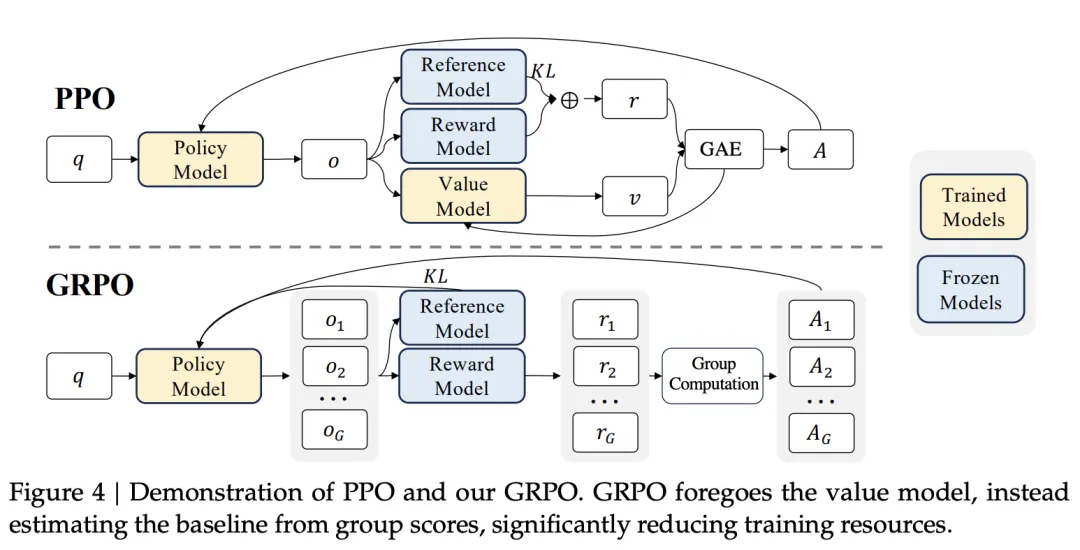
\includegraphics{images/image-0020.png}
\caption{PPO与GRPO架构对比}
\end{figure}

图中可以看出，PPO需要额外训练Value Model来估计价值基准，而GRPO冻结参考模型并使用组内样本奖励来估计Baseline，因此可以省去Critic网络。

\hypertarget{ux7fa4ux4f53ux91c7ux6837ux4ee3ux66ffux671fux671bux8ba1ux7b97}{%
\subsubsection{1. 群体采样（代替期望计算）}\label{ux7fa4ux4f53ux91c7ux6837ux4ee3ux66ffux671fux671bux8ba1ux7b97}}

对于每一个输入 \(q\)，我们使用旧策略 \(\pi_{\theta_{\mathrm{old}}}\) 采样一组共 \(G\) 个输出：

\[
\{o_1,o_2,\ldots,o_G\}\sim \pi_{\theta_{\mathrm{old}}}(O\mid q)
\]

随后，我们对每个输出计算奖励 \(\{r_1,r_2,\ldots,r_G\}\)。

\hypertarget{ux4f18ux52bfux4f30ux8ba1}{%
\subsubsection{2. 优势估计}\label{ux4f18ux52bfux4f30ux8ba1}}

这是GRPO取代Critic网络的关键。传统的A2C/PPO使用神经网络 \(V_{\phi}(s)\) 预测基准值，而在GRPO中，我们利用当前这组样本的平均奖励作为基准。

计算第 \(i\) 个样本的优势 \(A_i\)：

\[
A_i=\frac{r_i-\mu_{\mathrm{group}}}{\sigma_{\mathrm{group}}+\epsilon}
\]

其中 \(\mu_{\mathrm{group}}\) 表示当前组奖励均值，\(\sigma_{\mathrm{group}}\) 表示当前组奖励标准差。

除以标准差是因为考虑到不同类型的问题给分模式不同，可能互相不可比，故将其标准化。但也可能带来问题，比如对于过于难或简单的问题，几乎所有回答得分都一样时，该问题权重会被人为拉大。针对此问题后续已有工程上的优化。

\hypertarget{ux76eeux6807ux51fdux6570ux4e0eux957fux5ea6ux5f52ux4e00ux5316}{%
\subsubsection{3. 目标函数与长度归一化}\label{ux76eeux6807ux51fdux6570ux4e0eux957fux5ea6ux5f52ux4e00ux5316}}

目标函数 \(J(\theta)\) 如下：

\[
\mathcal{J}_{\mathrm{GRPO}}(\theta)=
\mathbb{E}_{q\sim P(Q),\{o_i\}_{i=1}^{G}\sim\pi_{\theta_{\mathrm{old}}}(O\mid q)}
\left[
\frac{1}{G}\sum_{i=1}^{G}\frac{1}{T_i}\sum_{t=1}^{T_i}
\left(
\min(\rho_{i,t}A_i,\mathrm{clip}(\rho_{i,t},1-\epsilon,1+\epsilon)A_i)-\beta D_{\mathrm{KL},t}
\right)
\right]
\]

这里Clip和KL同时存在，二者作用略有不同。Clip限制单次梯度更新的幅度，防止策略在一次迭代中变化过大导致训练崩塌；KL项保证最终策略距离初始参考策略不太远，关注累积效应，保证模型不会为了取得更高Reward而让语言能力退化。

这里 \(\rho_{i,t}\) 表示当前策略相对旧策略的概率比，\(D_{\mathrm{KL},t}\) 表示当前Token位置的KL惩罚项。对旧策略采样分布求期望后，可以得到策略和参考模型之间的KL约束；这里不需要遍历词表中的所有词，因为遍历通常是为了求期望，而组采样蒙特卡洛已经能近似得到该期望。

之所以用反向KL散度而非前向KL散度，是因为反向KL散度 \(KL(\pi_{\theta}\Vert\pi_{\mathrm{ref}})\) 会对当前策略高概率、参考策略低概率的区域给出较大惩罚，进而呈现``模式搜索''行为，让新的概率空间收敛到预训练后概率较大的空间里的特定模式（如果跳出空间往往表现为输出乱码、不符合正常语义的内容等，即``模式崩塌''）；前向KL散度则会倾向于覆盖预训练后的高概率空间，呈现``均值搜索''行为。RL获得的空间往往是预训练的子集（这也可能是RL难以让模型获得预训练完全没见过的技能的原因之一）。

方括号内，对于同一个输入，从第1到第 \(G\) 个输出取平均，然后是一个长度归一化项。这个长度归一化项是GRPO的另一个关键。

标准的策略梯度下，我们优化的目标是总奖励的期望：

\[
J=\mathbb{E}_{\tau\sim\pi_{\theta}}[R(\tau)]
\]

其梯度是（忽略Baseline）：

\[
\nabla J\approx \sum_{t=1}^{T}\nabla\log\pi_{\theta}(a_t\mid s_t)\cdot R
\]

目标函数 \(J\) 的梯度是对每一个动作的策略计算并累加的。假设 \(J\) 对每个动作的梯度大小为1，那么长为100的序列得到的梯度就约为长为10的序列的十倍，这会导致模型被长序列主导更新。但对于同一个问题而言，每个答案序列贡献的梯度应该是``平等''的，故我们需要除以序列长度 \(T\)：

\[
\nabla J_{\mathrm{GRPO}}\approx \frac{1}{T}\sum_{t=1}^{T}\nabla\log\pi_{\theta}(a_t\mid s_t)\cdot A
\]

但这也会产生一个问题，那就是当我们把 \(J\) 的梯度除以 \(T\) 时，意味着把目标函数 \(J\) 本身也除以了 \(T\)，目标函数变成了``单位Token能获得的奖励的期望''。这会导致模型在回答错误时生成大量无用的Token。原因在于：

当优势函数为正值时，意味着生成的结果是正确的，目标函数为正。由于目标函数是``单位Token能获得的奖励的期望''（有分母 \(T\)），为了让目标函数变大，策略在优化过程中会倾向于生成简短的正确答案，即这样的答案会产生比其他答案更大的梯度更新幅度。

当优势函数为负值时，意味着生成的结果是错误的，目标函数为负。为了让目标函数变大（惩罚的绝对值变小），策略会倾向于生成较长的答案（因为目标函数中除以较大 \(T\)），即这样的答案受到的负向惩罚和梯度压力反而更小。

\hypertarget{ux4e09ux4f18ux52bfux51fdux6570ux4f30ux8ba1ux7684ux6709ux504fux6027ux95eeux9898ux53caux89e3ux51b3ux65b9ux6848}{%
\subsection{三、优势函数估计的有偏性问题及解决方案}\label{ux4e09ux4f18ux52bfux51fdux6570ux4f30ux8ba1ux7684ux6709ux504fux6027ux95eeux9898ux53caux89e3ux51b3ux65b9ux6848}}

GRPO的优势函数估计看似是无偏的，实则往往对难题低估、对简单题高估。例如，一次取8条路径，对于一道答对概率只有1\%的难题，答对奖励为1，答错奖励为0，则8条路径都答错时没有梯度；有一条答对时，答对的那条路径优势函数为 \(1-\frac{1}{8}=\frac{7}{8}\)，但实际上优势函数为 \(1-\frac{1}{100}=\frac{99}{100}\)。对于简单题则相反，如答对概率为99\%，一条答错，答对者优势函数即为 \(\frac{1}{8}\)，实际上只有 \(\frac{1}{100}\)。

对此，可将难题优势函数乘以更大系数，简单题优势函数乘以更小系数，以尽可能实现无偏估计。

\hypertarget{ux53c2ux8003ux6587ux732e-83}{%
\subsection{参考文献}\label{ux53c2ux8003ux6587ux732e-83}}

\begin{itemize}
\tightlist
\item
  Shao, Z., Wang, P., Zhu, Q., et al.~(2024). \href{https://arxiv.org/abs/2402.03300}{DeepSeekMath: Pushing the Limits of Mathematical Reasoning in Open Language Models}. arXiv:2402.03300.
\end{itemize}

\clearpage

\hypertarget{klux6563ux5ea6ux7684ux9009ux62e9}{%
\section{KL散度的选择}\label{klux6563ux5ea6ux7684ux9009ux62e9}}

\hypertarget{ux4e00llmux4e2dux7684klux6563ux5ea6}{%
\subsection{一、LLM中的KL散度}\label{ux4e00llmux4e2dux7684klux6563ux5ea6}}

在大模型中，KL散度衡量输出概率分布的差异，并非按输出前的隐藏层维度计算，而是在大小为 \(V\) 的词表上计算（因为本质上大模型的输出是离散的tokens）。

\(D(P \Vert Q)=\sum_{i=1}^{V}p_i\log\frac{p_i}{q_i}\)，相当于 \(\log(p_i/q_i)\) 在 \(p\) 分布上的期望。

对于LLM，自回归输出 \(n\) 个token的KL散度：

\[
D_{KL}(P(Y) \Vert Q(Y))=\sum_Y P(Y)\log\frac{P(Y)}{Q(Y)}
\]

由于直接对所有可能的序列求和是不可行的（有 \(V^n\) 种可能），需利用自回归特性分解：

\[
\begin{aligned}
D_{KL}(P(Y) \Vert Q(Y))
&= \mathbb{E}_{Y\sim P}\left[\sum_{t=1}^{n}\left(\log P(y_t\mid y_{<t})-\log Q(y_t\mid y_{<t})\right)\right] \\
&= \sum_{t=1}^{n}\mathbb{E}_{Y\sim P}\left[\log\frac{P(y_t\mid y_{<t})}{Q(y_t\mid y_{<t})}\right]
\end{aligned}
\]

这里的处理难点在于 \(Y\sim P\)，需要考虑整个序列的概率分布。注意到右边的条件概率的条件为 \(y_{<t}\)，对于给定已知的 \(y_{<t}\) 分布，由自回归特性，\(y_t\) 的分布也会随之确定，\(Y=\{y_1,\ldots,y_t\}\) 的分布也就已知。因此可以改写为：

\[
D_{KL}(P(Y) \Vert Q(Y))
=\sum_{t=1}^{n}\mathbb{E}_{y_{<t}\sim P(y_{<t})}\left[
D_{KL}\left(P(y_t\mid y_{<t}) \Vert Q(y_t\mid y_{<t})\right)
\right]
\]

这意味着，两个序列分布的KL散度，等于每一步条件概率分布之间KL散度的期望之和（期望是基于分布P生成的历史轨迹计算的）。利用蒙特卡洛估计，在策略P下生成的各轨迹平均即可近似策略P下的期望。

\hypertarget{ux4e8ck1ux4f30ux8ba1ux5668ux548ck3ux4f30ux8ba1ux5668}{%
\subsection{二、K1估计器和K3估计器}\label{ux4e8ck1ux4f30ux8ba1ux5668ux548ck3ux4f30ux8ba1ux5668}}

对于长度为T的序列：

\textbf{K1 估计器（The Naïve Estimator）}

这是最直观的蒙特卡洛估计，直接计算 log 似然比：

\[
K1=\sum_{t=1}^{T}K1_t
=\sum_{t=1}^{T}\log\frac{\pi_\theta(y_t\mid x,y_{<t})}{\pi_{\mathrm{ref}}(y_t\mid x,y_{<t})}
\]

特点：它是 \(D_{KL}(\pi_\theta \Vert \pi_{\mathrm{ref}})\) 的无偏估计，但在实践中方差较大。

\textbf{K3 估计器（The Schulman Estimator）}

由 John Schulman 提出，旨在减少方差。它利用了 \(\log(x)\le x-1\) 的性质来逼近：

\[
K3=\sum_{t=1}^{T}K3_t
=\sum_{t=1}^{T}\left(
\frac{\pi_{\mathrm{ref}}(y_t\mid x,y_{<t})}{\pi_\theta(y_t\mid x,y_{<t})}
-1
-\log\frac{\pi_{\mathrm{ref}}(y_t\mid x,y_{<t})}{\pi_\theta(y_t\mid x,y_{<t})}
\right)
\]

特点：它也是 \(D_{KL}(\pi_\theta \Vert \pi_{\mathrm{ref}})\) 的无偏估计（期望为 KL 散度值），且具有比 K1 更低的方差。

KL散度项可以减在Reward或加在Loss里。在实际训练中，K1 in loss和K3 in reward不稳定，一般采用K3 in loss（方差更小）或K1 in reward（梯度无偏）。GRPO默认前者，但2025年有研究证明后者实际上可能性能更优，因为前者本身无偏但其梯度有偏。

\hypertarget{ux4e09ux8bc1ux660ek1-in-rewardux68afux5ea6ux65e0ux504fux53cak3-in-lossux68afux5ea6ux6709ux504f}{%
\subsubsection{（三）证明K1 in reward梯度无偏及K3 in loss梯度有偏}\label{ux4e09ux8bc1ux660ek1-in-rewardux68afux5ea6ux65e0ux504fux53cak3-in-lossux68afux5ea6ux6709ux504f}}

我们需要优化的真实目标（Reverse KL）的梯度为：

\[
\nabla_\theta D_{KL}(\pi_\theta \Vert \pi_{\mathrm{ref}})
=\mathbb{E}_{y\sim\pi_\theta}\left[
\log\frac{\pi_\theta}{\pi_{\mathrm{ref}}}\nabla_\theta\log\pi_\theta
\right]
\]

注：为简化符号，省略条件 \(x\) 和求和符号，关注核心各项。

\textbf{推导 1：K1 in Reward（无偏）}

当把 K1 放入 Reward 时，我们不对 K1 本身求导（视为常数奖励），而是利用 REINFORCE/PPO 的性质：

\[
\mathrm{Gradient}
=\mathbb{E}_{y\sim\pi_\theta}\left[K1\cdot\nabla_\theta\log\pi_\theta\right]
\]

代入 \(K1=\log\frac{\pi_\theta}{\pi_{\mathrm{ref}}}\)：

\[
\mathrm{Gradient}
=\mathbb{E}_{y\sim\pi_\theta}\left[
\left(\log\frac{\pi_\theta}{\pi_{\mathrm{ref}}}\right)
\nabla_\theta\log\pi_\theta
\right]
\]

结论：这与 Reverse KL 的真实梯度表达式完全一致，因此是无偏的。

\textbf{推导 2：K3 in Loss（有偏）}

当把 K3 放入 Loss 时，我们直接计算 \(\nabla_\theta K3\) 的期望。设比率 \(r=\frac{\pi_{\mathrm{ref}}}{\pi_\theta}\)，则 \(K3=r-1-\log r\)。注意 \(\log r=\log\pi_{\mathrm{ref}}-\log\pi_\theta\)。

我们需要计算 \(\mathbb{E}_{y\sim\pi_\theta}[\nabla_\theta K3]\)。首先看 \(\nabla_\theta K3\) 的各项：

\begin{enumerate}
\def\labelenumi{\arabic{enumi}.}
\tightlist
\item
  \(\nabla_\theta r=\nabla_\theta(\pi_{\mathrm{ref}}\cdot\pi_\theta^{-1})=\pi_{\mathrm{ref}}\cdot(-1)\pi_\theta^{-2}\cdot\nabla_\theta\pi_\theta=-\frac{\pi_{\mathrm{ref}}}{\pi_\theta}\cdot\frac{\nabla_\theta\pi_\theta}{\pi_\theta}=-r\nabla_\theta\log\pi_\theta\)
\item
  \(\nabla_\theta(-1)=0\)
\item
  \(\nabla_\theta(-\log r)=\nabla_\theta(\log\pi_\theta-\log\pi_{\mathrm{ref}})=\nabla_\theta\log\pi_\theta\)（假设 \(\pi_{\mathrm{ref}}\) 固定）
\end{enumerate}

合并各项得到 \(\nabla_\theta K3\)：

\[
\nabla_\theta K3
=-r\nabla_\theta\log\pi_\theta+\nabla_\theta\log\pi_\theta
=(1-r)\nabla_\theta\log\pi_\theta
\]

现在计算其期望：

\[
\mathbb{E}_{y\sim\pi_\theta}[\nabla_\theta K3]
=\mathbb{E}_{y\sim\pi_\theta}\left[(1-r)\nabla_\theta\log\pi_\theta\right]
\]

\[
\begin{aligned}
&=\mathbb{E}_{y\sim\pi_\theta}\left[\nabla_\theta\log\pi_\theta\right]
-\mathbb{E}_{y\sim\pi_\theta}\left[
\frac{\pi_{\mathrm{ref}}}{\pi_\theta}\nabla_\theta\log\pi_\theta
\right] \\
&=-\mathbb{E}_{y\sim\pi_\theta}\left[
\frac{\pi_{\mathrm{ref}}}{\pi_\theta}\nabla_\theta\log\pi_\theta
\right]
\end{aligned}
\]

其中第一项为 \(0\)（Score Function property）。

对比真实梯度：

\begin{itemize}
\tightlist
\item
  真实 Reverse KL 梯度：\(\mathbb{E}\left[\log\left(\frac{\pi_\theta}{\pi_{\mathrm{ref}}}\right)\nabla\log\pi_\theta\right]\)
\item
  K3 in Loss 梯度：\(\mathbb{E}\left[-\frac{\pi_{\mathrm{ref}}}{\pi_\theta}\nabla\log\pi_\theta\right]\)
\end{itemize}

事实上，K3估计器梯度变成了对应前向KL散度的梯度，而非反向KL散度，导致模型训练中更倾向于覆盖已有模式，而非在模式内部探索奖励最高区域。

其中Score Function property：

\textbf{1. 数学推导（The ``Why''）}

我们要证明的是：

\[
\mathbb{E}_{y\sim\pi_\theta}\left[\nabla_\theta\log\pi_\theta(y)\right]=0
\]

证明步骤如下：

\textbf{第一步：展开期望的定义}。期望 \(\mathbb{E}\) 就是对所有可能的 \(y\) 进行加权求和（对于离散的 LLM token 序列是求和，连续空间是积分）。

\[
\mathbb{E}_{y\sim\pi_\theta}\left[\nabla_\theta\log\pi_\theta(y)\right]
=\sum_y \pi_\theta(y)\cdot\nabla_\theta\log\pi_\theta(y)
\]

\textbf{第二步：应用对数求导法则（Log-Derivative Trick）}。根据微积分中的链式法则，\(\nabla\log f(x)=\frac{\nabla f(x)}{f(x)}\)。将其应用到 \(\log\pi_\theta(y)\) 上：

\[
\nabla_\theta\log\pi_\theta(y)
=\frac{\nabla_\theta\pi_\theta(y)}{\pi_\theta(y)}
\]

\textbf{第三步：代回并约分}。将第二步的结果代回第一步的式子中：

\[
\sum_y \pi_\theta(y)\cdot
\frac{\nabla_\theta\pi_\theta(y)}{\pi_\theta(y)}
=\sum_y \nabla_\theta\pi_\theta(y)
\]

\textbf{第四步：交换求和与求导的顺序}。在满足一定正则性条件下，我们可以交换求和符号 \(\sum\) 和梯度符号 \(\nabla_\theta\)：

\[
\sum_y \nabla_\theta\pi_\theta(y)
=\nabla_\theta\left(\sum_y \pi_\theta(y)\right)
\]

\textbf{第五步：利用概率归一化性质}。这是最关键的一步。对于任何概率分布，其所有可能事件的概率之和必须恒等于 1：

\[
\sum_y \pi_\theta(y)=1
\]

因此：

\[
\nabla_\theta\left(\sum_y \pi_\theta(y)\right)
=\nabla_\theta(1)=0
\]

所以：

\[
\mathbb{E}_{y\sim\pi_\theta}\left[\nabla_\theta\log\pi_\theta(y)\right]=0
\]

\textbf{2. 直观理解（The Intuition）}

``概率质量守恒''梯度 \(\nabla_\theta\pi_\theta(y)\) 代表当我们微调参数 \(\theta\) 时，样本 \(y\) 出现的概率是增加还是减少。

\begin{itemize}
\tightlist
\item
  如果我们让某些样本的概率增加了（梯度为正），那么为了保持总概率之和永远为 1，必然有另一些样本的概率要减少（梯度为负）。
\item
  这个式子 \(\mathbb{E}[\nabla\log\pi]=\sum\nabla\pi\) 实际上就是在计算所有可能样本的概率变化量的总和。
\item
  因为总概率（这个``蛋糕''的大小）是固定的 1，所以所有变化的加和必须为 0。
\end{itemize}

\hypertarget{ux53c2ux8003ux6587ux732e-84}{%
\subsection{参考文献}\label{ux53c2ux8003ux6587ux732e-84}}

\begin{itemize}
\tightlist
\item
  Schulman, J. (2020). \href{http://joschu.net/blog/kl-approx.html}{Approximating KL Divergence}.
\item
  Ziegler, D. M., Stiennon, N., Wu, J., et al.~(2019). \href{https://arxiv.org/abs/1909.08593}{Fine-Tuning Language Models from Human Preferences}. arXiv:1909.08593.
\item
  Ouyang, L., Wu, J., Jiang, X., et al.~(2022). \href{https://arxiv.org/abs/2203.02155}{Training language models to follow instructions with human feedback}. NeurIPS 2022.
\item
  Ahmadian, A., Cremer, C., Gallé, M., et al.~(2024). \href{https://arxiv.org/abs/2402.14740}{Back to Basics: Revisiting REINFORCE Style Optimization for Learning from Human Feedback in LLMs}. ACL 2024.
\end{itemize}

\clearpage

\hypertarget{ux4e3aux4ec0ux4e48online-rlux6bd4sftux66f4ux80fdux907fux514dux707eux96beux6027ux9057ux5fd8}{%
\section{为什么Online RL比SFT更能避免``灾难性遗忘''}\label{ux4e3aux4ec0ux4e48online-rlux6bd4sftux66f4ux80fdux907fux514dux707eux96beux6027ux9057ux5fd8}}

研究指出，On-Policy RL在避免``灾难性遗忘''上优于SFT（《RL'S RAZOR: WHY ONLINE REINFORCEMENT LEARNING FORGETS LESS》，MIT，2025）。相比于利用SFT微调，用On-Policy RL微调后的模型输出的策略与原预训练模型输出策略间的KL散度更小。（这里的KL散度工程上用的是在输入为新任务的情况下求出的期望，这是一个经验性的发现，即模型在新任务上的分布偏移量能预测它在旧任务上的遗忘程度；论文预测指标是Forward KL，但也指出RL之所以遗忘少，是因为它在优化过程中隐式地最小化了反向KL散度）

\hypertarget{ux4e00ux6838ux5fc3ux539fux56e0}{%
\subsection{一、核心原因}\label{ux4e00ux6838ux5fc3ux539fux56e0}}

SFT（Offline）：使用外部固定的数据集。这些数据的分布可能与模型当前的分布相去甚远。SFT 会强制将模型输出拉向这个任意的外部分布。由于解空间很大，外部数据往往会将模型引导至一个距离当前位置很远的最优解，导致剧烈的KL偏移，进而引发遗忘。论文发现，使用Off-Policy RL也存在类似问题。

RL（On-Policy）：使用模型自身生成的样本。On-Policy RL的更新逻辑是：对模型自己按当前策略生成的样本进行重加权，增加高奖励样本的概率，降低低奖励样本的概率。因为样本来自自身策略 \(\pi\)，RL的更新本质上是在当前分布的邻域内进行调整。它不会像SFT那样被强行拉向一个未知的、可能正交于原知识表示的分布。相反，On-Policy RL倾向于在满足新任务要求的前提下，寻找一条KL变化最小的路径。

\hypertarget{ux4e8cux4eceux6295ux5f71ux7684ux89c6ux89d2ux770brlux7684ux6536ux655b}{%
\subsection{二、从投影的视角看RL的收敛}\label{ux4e8cux4eceux6295ux5f71ux7684ux89c6ux89d2ux770brlux7684ux6536ux655b}}

标准的策略梯度方法本质上就是一个在``可行策略空间''和``最优解空间''之间，交替进行两种投影的算法：

假设我们处于一个简化的二值奖励（Binary Reward，\(R \in \{0,1\}\)）场景中：

\textbf{第一步：E-Step（I-Projection / 信息投影）}。这一步并不是在更新神经网络参数，而是在\textbf{构建目标分布}。当我们用当前策略 \(\pi_t\) 采样，并根据奖励 \(R\) 进行筛选（例如只保留 \(R=1\) 的样本，即 Rejection Sampling）时，我们实际上构建了一个新的非参数化分布 \(q_t\)。

论文证明（Lemma A.1），这个重加权后的分布 \(q_t\)，在数学上是所有满足``最优性条件''（即 \(\mathbb{E}_q[R]=1\)）的分布中，距离当前策略 \(\pi_t\) KL 散度最近的那一个：

\[
q_t = \arg\min_{q:\mathbb{E}_q[R]=1} D_{KL}(q\Vert \pi_t)
\]

直观理解：这相当于在``高分答案集合''中找一个离我现在怎么说话最像的分布。

\textbf{第二步：M-Step（M-Projection / 矩投影）}。这一步才是我们熟悉的梯度下降更新参数。当我们计算策略梯度 \(\nabla \mathbb{E}[R]\) 并更新 \(\pi\) 时，论文证明（Lemma A.2）这等价于让新的参数化策略 \(\pi_{t+1}\) 去拟合上述的理想分布 \(q_t\)。

这实际上是在最小化 \(D_{KL}(q_t\Vert \pi)\)（即交叉熵损失）：

\[
\pi_{t+1} = \arg\min_{\pi\in\Pi} D_{KL}(q_t\Vert \pi)
\]

直观理解：修改我的模型参数，让它尽可能模仿刚才那个``既得了高分又离我很近''的理想分布 \(q_t\)。

从而这种连续的投影过程最终收敛到的解，理论上是所有能完成任务（最优）的策略中，距离初始策略的KL散度最小的那一个。

\begin{figure}[htbp]
\centering
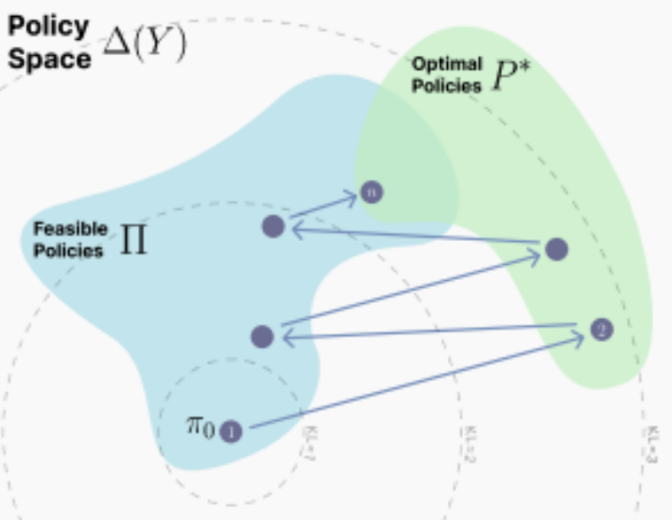
\includegraphics{images/image-0021.png}
\caption{Policy Space / Feasible Policies / Optimal Policies 概念图}
\end{figure}

下面证明这两步过程和On-Policy RL的等价性：

\hypertarget{ux7b2cux4e00ux6b65ux4e3aux4ec0ux4e48ux62d2ux7eddux91c7ux6837ux7b49ux4ef7ux4e8e-i-projection}{%
\subsubsection{第一步：为什么``拒绝采样''等价于 I-Projection？}\label{ux7b2cux4e00ux6b65ux4e3aux4ec0ux4e48ux62d2ux7eddux91c7ux6837ux7b49ux4ef7ux4e8e-i-projection}}

\textbf{结论：}从当前策略 \(p\) 中进行拒绝采样（Rejection Sampling），得到的分布 \(q_{RS}\)，正是满足``奖励约束''且距离 \(p\) KL 散度最小的分布。

\textbf{证明过程：}

\textbf{1. 定义场景：}

\begin{itemize}
\tightlist
\item
  \(p(y)\) 是当前策略（Base distribution）。
\item
  \(R(y) \in \{0,1\}\) 是二值奖励函数。
\item
  \(S=\{y\in Y:R(y)=1\}\) 是所有正确答案的集合（即获得奖励的样本）。
\item
  拒绝采样的过程是：从 \(p\) 采样，保留 \(y\in S\)。这产生的经验分布实际上就是条件概率分布 \(p(y\mid S)\)。
\end{itemize}

\textbf{2. 构建优化目标（I-Projection）：}我们需要寻找一个分布 \(q\)，使得它在满足期望奖励为 1 的前提下，与 \(p\) 最接近：

\[
\min_q D_{KL}(q\Vert p) \quad \mathrm{s.t.}\quad \mathbb{E}_{y\sim q}[R(y)] = 1
\]

\textbf{3. 推导等价性：}

约束条件 \(\mathbb{E}_{y\sim q}[R(y)]=1\) 意味着分布 \(q\) 的所有概率质量必须全部落在集合 \(S\) 上；如果 \(q\) 在非 \(S\) 区域有值，期望奖励就会小于 1。因此，\(q\) 的支持集（Support）必须包含在 \(S\) 内。

对于任意支持集在 \(S\) 上的分布 \(q\)，我们可以将 \(p(y)\) 分解为 \(p(y)=p(S)p(y\mid S)\)。代入 KL 散度公式：

\[
D_{KL}(q\Vert p)
= \sum_{y\in S} q(y)\ln\frac{q(y)}{p(y)}
= \sum_{y\in S} q(y)\ln\frac{q(y)}{p(S)p(y\mid S)}
\]

拆解对数项：

\[
D_{KL}(q\Vert p)
= \sum_{y\in S} q(y)\ln\frac{q(y)}{p(y\mid S)}
- \sum_{y\in S} q(y)\ln p(S)
\]

因为 \(\sum_{y\in S}q(y)=1\)，且 \(p(S)\) 是常数，第二项与 \(q\) 无关。第一项正是 \(D_{KL}(q\Vert p(\cdot\mid S))\)。

由 KL 散度的性质（\(D_{KL}\ge 0\)，当且仅当两个分布相等时为 0），要最小化上式，必须有 \(q(y)=p(y\mid S)\)。

也就是说当我们将RL中概率分布的调整简化为拒绝采样的情形后，它在数学上就严格等价于找到了一个理论上的最优目标分布。

\hypertarget{ux7b2cux4e8cux6b65ux4e3aux4ec0ux4e48ux7b56ux7565ux68afux5ea6ux7b49ux4ef7ux4e8e-m-projection}{%
\subsubsection{第二步：为什么``策略梯度''等价于 M-Projection？}\label{ux7b2cux4e8cux6b65ux4e3aux4ec0ux4e48ux7b56ux7565ux68afux5ea6ux7b49ux4ef7ux4e8e-m-projection}}

\textbf{结论：}使用策略梯度（Policy Gradient）更新参数化策略 \(\pi\)，等价于让 \(\pi\) 去拟合（投影到）上一步生成的目标分布 \(q\)。

\textbf{证明过程：}

\textbf{1. 定义目标分布：}设上一步得到的理想分布为 \(q(y)\)。在 RL 中，这通常是根据奖励重加权后的分布：

\[
q(y)=\frac{\pi_{\mathrm{old}}(y)R(y)}{Z}
\]

其中 \(Z\) 是归一化常数。

\textbf{2. 构建优化目标（M-Projection）：}我们需要找到一个新的参数化策略 \(\pi\)，使其尽可能接近理想分布 \(q\)：

\[
\min_\pi D_{KL}(q\Vert \pi)
\]

\textbf{3. 推导等价性：}

展开 KL 散度公式：

\[
D_{KL}(q\Vert \pi)
= \sum_y q(y)\ln\frac{q(y)}{\pi(y)}
= \sum_y q(y)\ln q(y)-\sum_y q(y)\ln\pi(y)
\]

第一项 \(\sum_y q(y)\ln q(y)\) 是目标分布的熵相关项，对于优化变量 \(\pi\) 来说是常数。因此，最小化 KL 散度等价于最大化第二项：

\[
\max_\pi \mathbb{E}_{y\sim q}[\ln \pi(y)]
\]

将 \(q(y)\) 的定义代回：

\[
\max_\pi \sum_y \frac{\pi_{\mathrm{old}}(y)R(y)}{Z}\ln\pi(y)
\]

忽略常数 \(Z\)，这等价于最大化：

\[
\mathbb{E}_{y\sim \pi_{\mathrm{old}}}[R(y)\ln\pi(y)]
\]

这正是标准策略梯度的一步更新目标。把采样分布固定为 \(\pi_{\mathrm{old}}\) 时，对 \(\mathbb{E}_{y\sim\pi_{\mathrm{old}}}[R(y)\ln\pi(y)]\) 求梯度，就得到策略梯度定理中的 \(R(y)\nabla\ln\pi(y)\) 形式。

策略梯度的更新过程，本质上就是在一个参数化的分布族中，寻找一个 \(D_{KL}(q\Vert \pi)\) 最小的解，让神经网络输出策略分布 \(\pi\) 尽可能拟合实际最优策略分布 \(q\)（但神经网络输出不可能总是完全和实际分布相同，故取不到零）。

这两个步骤共同构成了一个 EM 算法（Expectation-Maximization）的变体：

E-Step（I-Projection）：用拒绝采样隐式地构造出最优目标分布 \(q\)（非参数化的）。

M-Step（M-Projection）：用策略梯度更新参数 \(\pi\)，使其逼近 \(q\)。

正是因为每一步 M-Projection 都是在拉近 \(\pi\) 和 \(q\)（而 \(q\) 又是 \(\pi\) 自身的重加权），所以整个轨迹被约束在一条 KL 变化最小的路径上，从而避免了 SFT 那种因拟合外部分布而导致的剧烈参数漂移和遗忘。

\hypertarget{ux53c2ux8003ux6587ux732e-85}{%
\subsection{参考文献}\label{ux53c2ux8003ux6587ux732e-85}}

\begin{itemize}
\tightlist
\item
  Shenfeld, I., Pari, J., \& Agrawal, P. (2025). \href{https://arxiv.org/abs/2509.04259}{RL's Razor: Why Online Reinforcement Learning Forgets Less}. arXiv:2509.04259.
\end{itemize}

\clearpage
